% !TeX root = ../thesis.tex

% \documentclass[12pt]{article}   

% %\usepackage[latin9]{inputenc}
% \usepackage[margin=0.75in]{geometry}
% \usepackage{amsthm}
% \usepackage{amsmath}
% \usepackage{amssymb}
% \usepackage{amsrefs}
% \usepackage{graphicx}
% \usepackage{esint}
% \usepackage{hyperref}
% \usepackage{subfigure}
	


%\usepackage{fourier}
% \usepackage{xcolor} 
%\usepackage{epstopdf}

\renewcommand{\R}{{\mathbb{R}}}
\renewcommand{\Z}{{\mathbb{Z}}}
\renewcommand{\N}{{\mathbb{N}}}

\def\le{\leqslant}% lessoreqal
\def\ge{\geqslant}%greaterorequal

\newcommand{\re}{\mathrm{Re}}
\newcommand{\im}{\mathrm{Im}}
\renewcommand{\eps}{\varepsilon}
\newcommand{\e}{\varepsilon}

% \theoremstyle{plain}
% \newtheorem{lemma}{Lemma}[section]
% \newtheorem{proposition}{Proposition}[section]
% \newtheorem{theo}{Theorem}[section]
% \newtheorem{algo}{Algorithm}[section]
% \newtheorem{assump}{\bf{Assumption}}[section]
% \newtheorem{conj}{Conjecture}[section]
% \newtheorem{cor}{Corollary}[section]
% %% types roman
% \theoremstyle{remark}
% \newtheorem{remark}{\bf{Remark}}[section]
% \theoremstyle{remark}
% \newtheorem{example}{\bf{Example}}[section]
% \theoremstyle{remark}
% \newtheorem{definition}{\bf{Definition}}[section]

% \newcommand{\zz}[1]{\textbf{\textcolor{blue}{ZZ: #1}}}

% \title{Explicit and implicit TVD schemes for conservation laws with Caputo derivatives}
% \author{Jian-Guo Liu\thanks{Department of Mathematics and Department of Physics, Duke University, Box 90320, Durham NC 27708, USA (jliu@phy.duke.edu)}, \, \, Zheng Ma\thanks{Department of Mathematics,
% Shanghai Jiao Tong University,
% 800 Dongchuan RD, Shanghai, 200240, China (mayuyu@sjtu.edu.cn)}, \, \, Zhennan Zhou\thanks{Department of Mathematics, Duke University, Box 90320, Durham NC 27708, USA (zhennan@math.duke.edu)}}
% \date{} % Activate to display a given date or no date (if empty),
%          % otherwise the current date is printed 

% \begin{document}
% \maketitle

% \begin{abstract}
% In this paper, we investigate numerical approximations of  the scalar conservation law with the Caputo derivative, which introduces the memory effect.  We construct the first order and the second order explicit upwind schemes for such equations, which are shown to be conditionally $\ell^1$ contracting and TVD. However, the Caputo derivative leads to the modified CFL-type stability condition, $ (\Delta t)^{\alpha} = O(\Delta x)$, where $\alpha \in (0,1]$ is the fractional exponent in the derivative. When $\alpha$ is small, such strong constraint makes the numerical implementation extremely impractical. We have then proposed the implicit upwind scheme to overcome this issue, which is proved to be unconditionally $\ell^1$ contracting and TVD. Various numerical tests are presented to validate the properties of the methods and provide more numerical evidence in interpreting  the memory effect in conservation laws. 
  
% \end{abstract}
\chapter{带Caputo导数的分数阶守恒律方程的显示与隐式TVD算法}
%\section{Introduction}
%\citen{Xu:2007eaba}


% In this paper, we study numerical approximations to the scalar conservation law with Caputo derivatives. The governing equation is  the following conservation law with fractional time derivative:
在本章中,我们将研究时间方向为Caputo导数的标量守恒定律的数值近似。控制方程是以下分数阶时间导数的守恒律:
\begin{equation}\label{eq:main}
\partial_t^\alpha u(x,t) + f(u(x,t))_x = 0, \quad  x\in\R, \,\, t>0,
\end{equation}
% $u(x,t)$ is a certain density function or concentration, and $f(u)$ is the flux function. This equation is completed by an initial condition:
$u(x,t)$是密度或浓度函数,$f(u)$是通量。方程的初值为:
\begin{equation}
u(x, 0) = u_0(x), \quad x\in\R.
\end{equation}
这里,当$\alpha\in (0,1)$时,$\partial_t^\alpha$为所谓的Caputo导数(分数阶导数):
\[
\partial_t^\alpha u(t)=C_\alpha \int_0^t (t-s)^{-\alpha} \partial_s u(s)ds,
\]
其中$C_\alpha=1/\Gamma(1-\alpha)$。当$\alpha=1$时,$\partial_t^\alpha u (t)$即为通常的导数$\partial_t u(t)$。

% The Caputo derivative was introduced in \citen{Caputo} for diffusion of fluids in porous media with the memory effect.  It has been shown that the Caputo derivative is effective in modeling plasma transport (see \citen{Plasma1,Plasma2}), and fractional functions have been made use of to construct physics models for long--range or nonlocal interactions in space and time, see for e.g., \citen{MeltzlerKlafter,Zaslavsky}. Recently in \citen{Caffarelli},  Allen, Caffarelli and Vasseur proved the existence of the weak solutions and the H\"older continuity for such solutions when with both a fractional potential pressure and fractional time derivative. The scalar conservation law with Caputo derivatives \eqref{eq:main} models the time evolution of a distribution of interest with general flux function and memory effect.  However, while the physical interpretation is clear, not much mathematical research has been done for such equations.
Caputo导数最早在文献\citen{Caputo}中被引入,用于描述在具有{\it 记忆效应}的多孔介质中的扩散。一些之前的工作已经表明,Caputo导数对等离子体传输的建模是有效的(参见\citen{Plasma1,Plasma2}),并且已经利用分数函数来构建空间和时间中长距离或非局部相互作用的物理模型, 参见例如\citen{MeltzlerKlafter,Zaslavsky}。最近在\citen{Caffarelli}中,Allen,Caffarelli和Vasseur证明了当有分数势能压力和分数时间导数时,该方程的弱解是存在的并且是H\"older连续的。带有Caputo导数的标量守恒定律方程\eqref{eq:main}描述了具有一般通量函数和记忆效应的分布进行的时间演化,虽然相关的物理解释很清楚,但是对于这种方程并没有太多的数学研究。


% In the aspect of numerical approximation, many numerical methods have been introduced and analyzed for ODE's or diffusion equations with the Caputo derivative, see e.g., \citen{Xu:2013jjba,Xu:2007eaba,Zhao:2015gfba,Cao2013154,Kumar20062602}, and most of which can be extended to fractional space-time advection-diffusion equations (see \citen{LZATB}) with additional treatment in the space (fractional) derivatives.  Also, there have been a few worthy studies in numerical approximations of fractional space-time advection-dispersion equation, see \citen{ZLPM}. It has been shown in different equations that, a consistent discretization of   the Caputo derivative will introduce dissipation in time, which can help stabilize a numerical scheme. Therefore, at least for linear equations, the Caputo derivative does not cause extra challenges in numerical approximations. In \citen{Zhao:2015gfba}, Zhao, Sun and Karniadakis proposed  a numerical method to approximate viscous Burgers' equation, however the methods suffered from the Gibbs phenomenon at jumps since the Fourier collocation method was used for the space discretization. To our best knowledge, this was still the only successful attempt for nonlinear conservation laws, although the presence of the diffusion terms helped avoid the issue of weak solution.
在数值近似方面,已经有很多数值方法被提出,对带有Caputo导数的ODE或扩散方程也进行了大量分析,参见例如\citen{Xu:2013jjba,Xu:2007eaba,Zhao:2015gfba,Cao2013154,Kumar20062602}。其中大多数可以推广到分数阶时空平流扩散方程(参见\citen{LZATB}),对空间(分数阶)导数中进行了特殊处理。此外,对于分数时空对流--扩散方程的数值近似,已经有一些值得研究的参考文献,参见\citen{ZLPM}。在不同的方程中的研究已经表明,Caputo导数的相容的离散将引入时间耗散,这有助于稳定数值格式。因此,至少对于线性方程,Caputo导数不会在数值近似中引起额外的挑战。在\citen{Zhao:2015gfba}中,Zhao,Sun和 Karniadakis提出了一种逼近粘性Burgers方程的数值方法,但是由于他们将傅里叶配点法应用于空间离散化,所以得到的解在间断处出现了吉布斯现象。据我们所知,这仍然是分数阶非线性守恒定律目前唯一的尝试。

% In this paper, we aim to construct and analyze explicit and implicit upwind schemes for the scalar conservation law with the Caputo derivative  \eqref{eq:main}. We propose the first order and the second upwind schemes to equation \eqref{eq:main}, and show that with modified CFL conditions, the numerical schemes are TVD. However, the modified CFL conditions are becoming more restricted as $\alpha \rightarrow 0$, which makes the explicit schemes not feasible for small $\alpha$. Motivated by this, we further design an implicit upwind method for the conservation law which is shown to be $\ell^1$ contracting and thus TVD. And in particular, for the linear advection case, we also show that the implicit scheme is also energy stable and satisfies the entropy condition.
在本章中,我们的目的是对带有Caputo导数的标量守恒律方程\eqref{eq:main}构建显式和隐式迎风格式并进行分析。我们提出了方程\eqref{eq:main}的一阶和二阶格式,并且显示了在修改的CFL条件下,数值格式是全变差下降的(total variation diminishing,TVD)。然而,由于修改的CFL条件当$\alpha \rightarrow 0$时过于严格,这使得显式格式对于小的$\alpha$不可行。在此基础上,我们进一步设计了一种隐式的迎风格式,并且证明了该格式的$\ell^1$范数递减,因此是TVD的。特别地,对于线性对流的情况,我们还表明隐式格式也是能量稳定的,并满足熵条件。

% The rest of the paper is outline as follows. We summarize some preliminary knowledge of the scalar conservation law with the Caputo derivative in the second part of this section. In Section 2, we briefly summarize existing results on numerical approximation of the Caputo derivative. We first propose and show stability analysis of the first order and the second order explicit upwind scheme in Section 3, which is followed by the introduction of an implicit upwind scheme to avoid the CFL conditions. We carry out various numerical tests in Section 4, not only to verify the properties of the proposed schemes, but also investigate the interpretations of the Caputo derivative  by conducting some designed tests.
本章的其余部分概述如下。 我们在本节的第二部分总结了带Caputo导数的标量守恒定律的一些初步知识。 在第2节中,我们简要总结了Caputo导数的近似值的现有结果。 我们首先提出并展示了第3节第一阶和第二阶明显逆风方案的稳定性分析,然后引入了一种隐性的逆风方案来避免CFL条件。 我们在第4节进行各种数值测试,不仅要验证拟议方案的性质,还要通过进行一些设计的测试来调查Caputo导数的解释。

\section{基本知识和定义}
% In this part, we start by introducing the Mittag-Leffler function for the time fractional linear advection equation and conclude with discussions on weak solutions to the nonlinear conservation law with the Caputo derivative. We consider the following equation with fractional time derivative
在这部分中,我们首先介绍时间为分数阶导数的对流方程的Mittag-Leffler函数,并用Caputo导数讨论了非线性守恒律的弱解。我们考虑以含分数阶时间导数的方程
\begin{equation}\label{eq:FT}
\partial_t^\alpha u = -A u,\quad u(x,0)=g(x).
\end{equation}
$A$是一个某个给定的算子。根据拉普拉斯变换,
% By the standard Laplace transformation,
\[
\mathcal L u(s):=\hat u(s)= \int_0^\infty e^{-st} u(t)dt,
\]
方程\eqref{eq:FT}变成
\[
(s^\alpha + A)\hat u = s^{\alpha-1} g. 
\]
由拉普拉斯逆变换
\begin{equation}
u(t)=E_\alpha (-t^\alpha A) g,
\end{equation}
$E_\alpha(z)$是Mittag-Leffler函数
\begin{equation}
E_\alpha(z)=\sum_{n=0}^\infty \frac{z^n}{\Gamma (\alpha n+1)}.
\end{equation}
如果令$A = -a\partial_x$,其中$a$为常数,则相应的对流方程为,
\begin{equation}
\partial_t^\alpha u + a\partial_x u = 0,
\end{equation}
它的解可以写为
\begin{equation}
u(x,t) = \sum_{n=0}^\infty \frac{\partial_x^{n} g}{\Gamma(\alpha n + 1)}a^n t^{\alpha n}.
\end{equation}
%\zz{how is $\partial_x^{\alpha n}$ defined?}
% Notice that, when $\alpha = 1$, the equation reduces to the normal scalar conservation law, and from the above equation we get nothing but
注意,当$\alpha =1$时,该方程即变成通常的标量守恒律方程以及它的解
\begin{equation}
u(x,t) = g(x+at) = \sum_{n=0}^\infty \frac{\partial^n_x g}{n!} a^n t^n.
\end{equation}

%\subsection{Weak solutions}
% However, for general conservation laws \eqref{eq:main}, there is lack of representations, and it is more convenient to work with its weak solutions due to the nonlinear flux. We give the following definition:
然而,对于一般守恒定律\eqref{eq:main},由于非线性的通量使得解不能够显式表示,使用弱解更方便。 我们给出以下定义:
\begin{defn}\label{def_ws}
	$u(x,t)$是方程\eqref{eq:main}的{\it 弱解},如果$\partial_t^\alpha u\in L^1_{\mathrm{loc}}(\R)$,$f(u)\in L^1_{\mathrm{loc}}(\R)$及对于任何测试函数$\phi \in \mathcal{D}(\R)$,有
	\begin{equation}
	\int_\R \left(\partial_t^\alpha u \phi - f(u)\partial_x\phi\right)\,dx = 0.
	\end{equation}
\end{defn}
% One can easily verify that the notion of a weak solution extends that of a classical solution: every classical solution of (\ref{eq:main}) is also a weak solution.
人们可以很容易地验证弱解的概念是到经典解的推广:(\ref{eq:main})的每个经典解都是弱解。

%\subsection{Non-uniqueness for the Cauchy problem}
% However, like standard conservation laws, the weak solutions to  \eqref{eq:main} may not be unique. To construct a Cauchy problem which admits more than one weak solution, we choose the fractional Burgers' equation
然而,像标准守恒律一样,\eqref{eq:main}的弱解可能不唯一。 为了说明这点,我们考虑如下分数阶的Burgers'方程
\begin{equation}\label{burgers}
	\partial_t^\alpha u + \partial_x\left(\frac{1}{2}u^2\right) = 0,
\end{equation}
及初值
\begin{equation}
	u(x,0) = \begin{cases}
		1, \quad & x > 0, \\
		-1, \quad & x < 0.
	\end{cases}
\end{equation}

% First we claim that the initial data itself serves as one weak solution,  which means we have a static discontinuous solution, (see Figure \ref{non_uniq} left)
首先初值本身就是一个弱解,这意味着我们有一个静止的间断解(见图\ref{non_uniq}左)
\begin{equation}
u(x,t) = \begin{cases}
1, \quad & x > 0, \\
-1, \quad & x < 0.
\end{cases}
\end{equation}
% We now verify that this solution satisfies definition of the weak solution. First, we have
我们来验证这个解满足弱解的定义。首先,我们有
\[
\partial_t^\alpha u \equiv 0 \quad\mbox{for } \forall x\ne 0,
\]
同时还有
\[
f(u) = \frac{1}{2}u^2 \equiv \frac{1}{2} \quad\mbox{for } \forall x \ne 0.
\]
根据{\bf 定义}\ref{def_ws},对于每个``测试''函数$\phi\in\mathcal{D}(\R)$
\[
\int_\R \left(\partial_t^\alpha u \phi - f(u)\partial_x\phi\right)\,dx = 0 - \frac{1}{2}\int_\R \phi_x\,dx = 0.
\]
% So it's a weak solution of equation (\ref{burgers}). But obviously, this is not an entropy solution since the characteristics are moving outwards from the discontinuous jump.
所以这是方程(\ref{burgers})的一个弱解。但是显然,这不是一个熵解,因为特征线从间断处向外移动。

% To construct another solution, we use the numerical method we will introduce later in this paper,  and the numerical result is plotted in Figure \ref{non_uniq} right for $t=0.02$ and $\alpha=0.8$.
为了构建另一个解,我们使用我们将在本章稍后介绍的数值方法,数值结果绘制在图\ref{non_uniq}右侧,$t = 0.02$和$\alpha = 0.8$。
%\zz{please add time and $\alpha$} 
% We see that, intuitively, the solution is between the static discontinuous solution and the standard rarefaction solution, which manifests the memory effect. 
我们看到,直观地,该解处在静态不连续解和标准稀疏解之间,这表现出了记忆效应。
%\zz{for the right picture: 1. use the same plot domain as left. 2. draw a dashed line of rarefaction solution when $\alpha=1$ for comparison.}
\begin{figure}[htbp]
	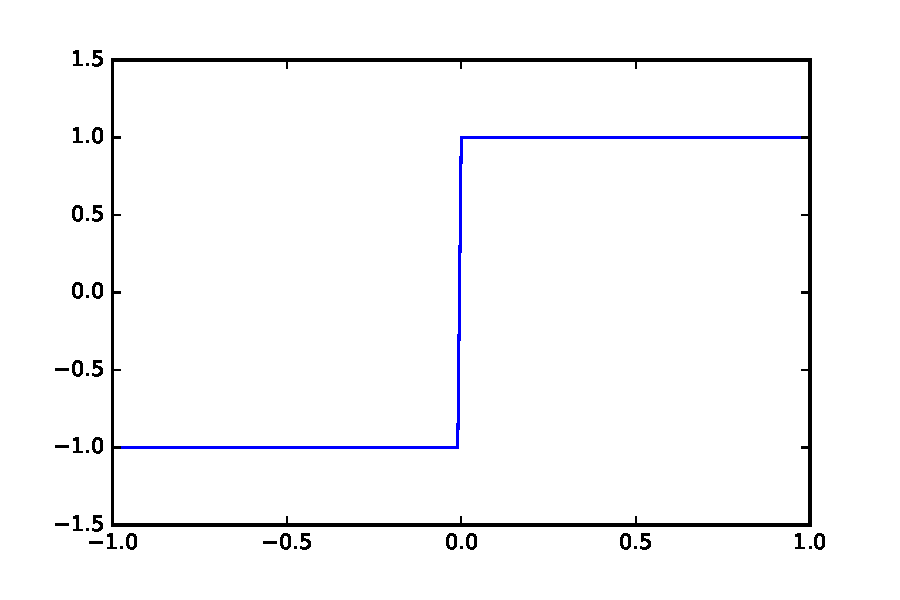
\includegraphics[width=0.5\textwidth]{frac_time/non_uniq_0}
	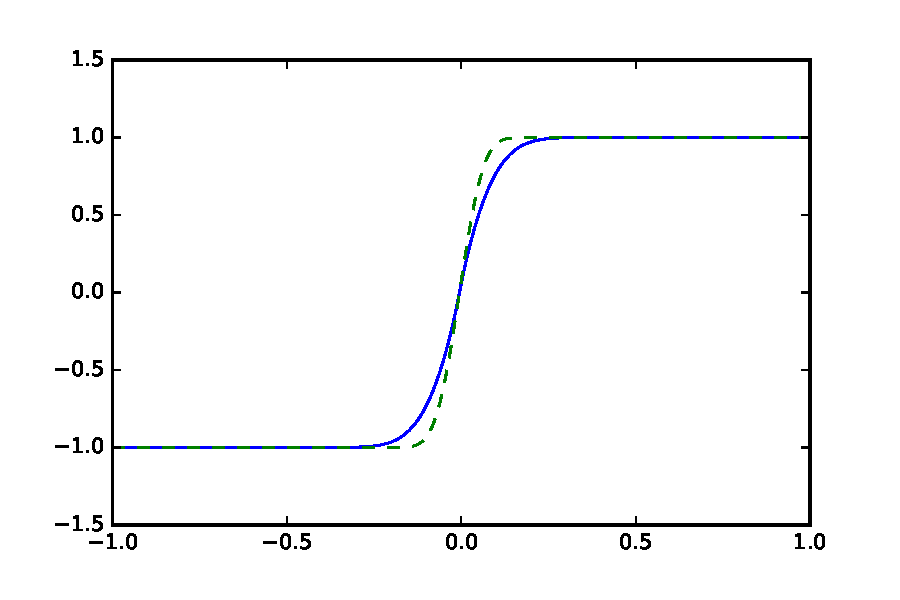
\includegraphics[width=0.5\textwidth]{frac_time/non_uniq}	
	\bicaption[non_uniq]{弱解不唯一性。左:静态的间断解;右:实线为带记忆效应的稀疏解,虚线普通为Burgers'方程的稀疏解。}{弱解不唯一性。左:静态的间断解;右:实线为带记忆效应的稀疏解,虚线普通为Burgers'方程的稀疏解。}{Fig}{Non-uniqueness of the solution. Left: the static discontinuous solution. Right: solid line is the rarefaction solution with memory effect; dashed line is the rarefaction solution for the Burgers' equation with the standard time derivative.}
	% \label{non_uniq}
\end{figure}

%\subsection{Entropy solutions}
% In order to define the entropy solutions, we consider the conservation law with artificial viscosity
为了定义熵解,我们考虑了具有人工粘性的守恒律
\begin{equation}\label{viscousity}
\partial_t^\alpha u + \partial_x f(u) = \varepsilon \partial_{xx} u.
\end{equation}
% Here, $\varepsilon>0$ is a diffusion coefficient, $\varepsilon\ll 1$. The Cauchy problem for (\ref{viscousity}) can be shown to have one and only one classical solution $u^\varepsilon$ which satisfies the maximum principle. If the sequence $\{u^\varepsilon\}$ converges almost everywhere to a function $u$ when $\varepsilon\to 0$, we call that $u$ is an entropy solution of (\ref{eq:main}). 
这里,$\varepsilon>0$是扩散系数,$\varepsilon\ll 1$。可以证明,(\ref{viscousity})的Cauchy问题具有满足最大原理的唯一一个经典解$u^\varepsilon$ 。 如果当$\varepsilon \to 0$时,序列$\{u^\varepsilon\}$收敛到函数$u$,我们称$u$是方程(\ref{eq:main})的熵解。

% We conclude this section by the following remark. It is entirely possible for one to define the entropy solutions by constructing the convex entropy function and entropy flux pairs and link that to the vanishing viscosity limit, but that will be quite analysis involved and is off the focus of the current paper. We will save the rigorous analysis of the entropy solutions to \eqref{eq:main} as one of the possible future directions. 
我们指出,通过构建一对函数,即凸熵函数和熵通量来定义熵解是完全有可能的,其粘性极限的定义是等价的,但这将涉及到大量分析,并不是本章的重点。


%%%%%%%%%%%%%%%%%%%%%%%

\section{Caputo导数的数值逼近}

%\zz{you need to rewrite the whole section with citing ref's and presenting main results in thm's}
%\subsection{Discretization}

% While there has been thorough understanding on numerical approximation of standard ordinary differential equations, the investigation of numerical methods for fractional ODEs (FODEs) is quite limited since rigorous numerical analysis of numerical methods of FODEs has met additional difficulties. However, there has been a growing interest in the research of this area. 
虽然人们对标准的常微分方程的数值近似有了深入的了解,但是由于分数阶时间导数的常微分方程(FODE)数值方法的严格分析会遇到额外的困难,因此对分数阶时间导数的ODE(FODE)数值方法的研究非常有限。但是最近人们对于这个研究领域的兴趣逐渐增加。

% Langlands and Henry \citen{Langlands2005719} considered the diffusion equation with fractional order time derivatives, and introduced an $L_1$-stable scheme for this equation. Sun and Wu \citen{SUN2006193} constructed a finite difference scheme with $L_1$ approximation for the fractional time derivative. Lin and Xu \citen{Xu:2007eaba} analyzed a finite difference scheme for the time discretization of the time fractional diffusion equation, and proved that the convergence in time is of $2-\alpha$ order. Lv and Xu \citen{LvXu} improved the error estimates by giving a more accurate coefficient. Zhao, Sun and Karniadakis \citen{Zhao:2015gfba} derived two second-order approximation formulas for fractional time derivatives involved in anomalous diffusion and wave propagation. Lin and Liu \citen{Lin2007856} analyzed a linear multistep method and proved the stability and convergence of the method. Kumar and Agrawal \citen{Kumar20062602} proposed  another numerical approach for a class of FODEs, which can be reduced into a Volterra type integral equation. Based on this approach, Cao and Xu \citen{Cao2013154} presented a general technique to construct high order numerical schemes for FODEs. 
Langlands和Henry\citen{Langlands2005719}考虑了具有分数阶时间导数的扩散方程,并为此方程引入了$ L_1 $稳定的数值格式。Sun和Wu\citen{SUN2006193}为分数阶时间导数构造了一个$L_1$近似的有限差分格式。Lin和Xu\citen{Xu:2007eaba}分析了分数阶扩散方程的时间离散化的有限差分格式,并证明了时间的收敛是$2-\alpha$阶。Lv和Xu\citen{LvXu}通过给出更准确的系数改进了误差估计。Zhao,Sun和Karniadakis\citen{Zhao:2015gfba}导出了涉及异常扩散和波传播的分数阶时间导数的两个二阶近似公式。Lin和Liu\citen{Lin2007856}分析了线性多步法,证明了该方法的稳定性和收敛性。Kumar和Agrawal\citen{Kumar20062602}提出了FODE的另一类数值方法,可以将其化减为Volterra型积分方程。基于这种方法,Cao和Xu\citen{Cao2013154}提出了一种构建FODE高阶数值方案的一般技术。

% In this paper, we use the following numerical approximation of the Caputo derivative, which basically follows the work done by  Lin and Xu in \citen{Xu:2007eaba}. We assume uniform time step size $\tau$, and denote $t^n=n\tau$, $n=0,1,2,\cdots$. We denote numerical approximation of $u(t^n)$ by $U^n$.
在本章中,我们使用如下Caputo导数的数值逼近(见\citen{Xu:2007eaba})。假设对于均匀的时间步长$\tau$,记$t^n=n\tau$, $n=0,1,2,\cdots$,$u(t^n)$的数值逼近记为$U^n$。为了构建一阶格式,假设

% To construct a first order method, for $t=t^{n+1}$,  we assume uniform partition in time,
\[
0=t_0<t_1<\cdots<t_n<t_{n+1}=t.
\]
% Afterwards, each standard time derivative is approximated by the forward difference. 
时间导数用向前差分逼近,即
% That is, 
\begin{align}
\partial_t^\alpha u (t^{n+1}) & \approx \frac 1 {\Gamma (1-\alpha)} \sum_{k=0}^n \int_{t_k}^{t_{k+1}} \frac{U^{k+1} - U^{k}}{
\tau(t_{n+1}-s)^\alpha}\,ds 
\nonumber \\
& =  \frac 1 {\Gamma (1-\alpha)(1-\alpha)} \sum_{k=0}^n \frac{(n+1-k)^{1-\alpha}-(n-k)^{1-\alpha}}{\tau^\alpha} (U^{k+1}-U^k) \nonumber \\
& =  \frac{1}{\Gamma(2-\alpha)\tau^\alpha} \left(U^{n+1}- \sum_{n=0}^k c^{n+1}_k U^k\right):=D_t^\alpha U^{n+1}, \label{eq:Cdev}
\end{align}
其中
\[
c^{n+1}_k = 2(n+1-k)^{1-\alpha}-(n+2-k)^{1-\alpha}-(n-k)^{1-\alpha}, \quad k=1,\cdots,n.
\]
\[
c^{n+1}_0=(n+1)^{1-\alpha}-n^{1-\alpha}.
\]
% By direct calculation, and note that $y=x^{1-\alpha}$ is an increasing and concave function for $x>0$, we get,
直接计算并注意到$y=x^{1-\alpha}$是单调递增的凹函数,有
\begin{equation}\label{cond:ck}
\sum_{k=0}^n c^{n+1}_k=1,\quad c^{n+1}_k >0, \quad k=0,\cdots,n.
\end{equation}
% Hence, while the standard time derivative gives the instantaneous rate of change, from its numerical approximation, from \eqref{eq:Cdev}, the Caputo derivative can be interpreted as the rate of change of a quantity from a convex combination of its history values, and the coefficients $c_k^{n+1}$ specifies the influence strength due to the memory effect. And the influence strength of a history values decreases in time since its memory effect becomes weaker. 
因此,正如标准时间导数可以给出瞬时变化率一样,从其数值近似,及\eqref{eq:Cdev}得出,Caputo导数可以被解释为从其历史值的凸组合中的量的变化率,并且系数$c_k^{n + 1}$表示出由于记忆效应引起的影响的强度。历史的影响随着记忆效应的变弱而逐渐减小。

% It is worth remarking that, we have for fixed $\alpha$,
值得指出,对于固定的$\alpha$,
\[
c^{n+1}_n=2-2^{1-\alpha}-0^{1-\alpha}=2-2^{1-\alpha},
\]
独立于$n$。因此,我们记$c^{n+1}_n$为$\tilde c$,它将是显式迎风格式的CFL中一个重要的量,将在后面予以说明。

% The consistency error has been proved by Lv and Xu \citen{LvXu}, which is the following Theorem, 
相容性误差由Lv和Xu在\citen{LvXu}中证明,如下述定理,
\begin{lem}
对于任意$\alpha\in(0,1)$,这个格式的截断误差为,
\begin{equation}
\partial^\alpha_{t} u (t^{n}) = D_t^\alpha u (t^{n})+ r^{n}_{\tau},
\end{equation}
满足如下误差估计
\begin{equation}
|r^k_\tau| \le CM(u)\tau^{2-\alpha}, \quad \forall k=0,1,\cdots, n,
\end{equation}
$C$独立于$u$和$\tau$,$M(u) = \max\limits_{t\in (0,t^n]}|\partial_t^2 u(t)|$.
\end{lem} 

% It is worth remarking that, the focus of the current paper is to construct and analyze numerical methods for conservation laws with the Caputo derivative, so we choose to use a prevailing method for numerical approximation of the Caputo derivative.  Actually, since many higher order approximation are available for the Caputo derivative, (see, e.g. \citen{Zhao:2015gfba,Cao2013154}), the accuracy in time of the numerical methods proposed in the following can easily be improved  with these results. 
值得指出的是,本章的重点是用Caputo导数构建和分析守恒律的数值方法,所以我们选择使用了一个常见的Caputo导数的数值近似。实际上,由于Caputo导数有许多较高阶的近似(参见,例如\citen{Zhao:2015gfba,Cao2013154}),以下结果和提出的数值方法的时间精度可以很容易地改善。
%%%%%%%%%%%%%%%%%%%%%%%


\section{数值方法和稳定性分析}

% In this section, we utilize the numerical approximation of the Caputo derivative introduced in the previous section to design numerical schemes for ODE's and conservation laws.  We focus on the stability condition for each scheme, especially how they differ from the models with standard time derivatives.
在本节中,我们利用上一节介绍的Caputo导数的数值近似来设计FODE和守恒定律的数值格式。我们专注于每个格式的稳定性条件,特别是它们与标准时间导数的模型不同之处。
\subsection{FODE模型的向后欧拉格式}
考虑如下ODE模型
\begin{equation}\label{mod:ode}
\partial_t^\alpha u(t)=\lambda u(t).
\end{equation}
$\lambda$为复数${\bf Re} (\lambda) \le 0$,表示离散算子的特征值。

% The stability analysis of several numerical schemes for ODE models with Caputo derivatives have been shown in some previous works, see~\citen{Xu:2013jjba,Xu:2007eaba,LvXu,xu2014alternating,gao2015three}. However, in this work, since we aim to design fully implicit schemes for nonlinear conservations laws in  Section 3.3, we need to utilize the numerical methods for the ODE models where the time discretization is given by a backward differentiation formula (BDF), which have not been studied yet.  Thus, we start by considering the backward Euler method for such ODE models.
Caputo导数的ODE模型的几个数值方案的稳定性分析已经在以前的一些文献中有所提及,见\citen{Xu:2013jjba,Xu:2007eaba,LvXu,xu2014alternating,gao2015three}。 然而,在这项工作中,由于我们的目标是设计非线性守恒律的全隐式格式,所以我们需要利用ODE模型的数值方法,其中时间离散化由后向微分公式(BDF)给出, 而这个工作尚未有人研究。因此,我们首先考虑这种ODE模型的向后欧拉方法。
\begin{equation}\label{backE}
D_t^\alpha U^{n+1}=\lambda U^{n+1}.
\end{equation}
两边同乘$\tau^{\alpha}\Gamma (2-\alpha)$得到
\[
\left(1-\lambda\tau^\alpha\Gamma(2-\alpha) \right)U^{n+1} = \sum_{k=0}^{n} c_k^{n+1} U^{k}.
\]
如果记$z=\lambda\tau^\alpha\Gamma (2-\alpha)$,格式对应的稳定多项式$\pi(\xi;z)$
\[
\pi(\xi;z)=\left(1-z \right)\xi^{n+1} - \sum_{k=0}^{n} c^{n+1}_k \xi^{k}.
\]

% In the following, we discuss two different situations, i.e., when $\lambda \ne 0$ and when $\lambda=0$.
下面考虑两种情况,即当$\lambda \ne 0$和当$\lambda=0$时,

当$\lambda \ne 0$时,${\bf Re} (z) \le 0$,$z\ne 0$,可以得到
$|1-z|>1$.
假设$\xi_0$及$|\xi_0|\ge1$是$\pi(\xi;z)$的根,对于$k\le n$有,
\[
|\xi_0^k| \le |\xi_0|^k \le |\xi_0^{n+1}|.
\]
可以得到
\begin{align*}
|(1-z)\xi_0^{n+1}|& = |1-z||\xi_0|^{n+1 }=|\sum_{k=0}^n c^{n+1}_k \xi_0^k| \\
& \le \sum_{k=0}^n c^{n+1}_k |\xi_0|^k  \le \left( \sum_{k=0}^n c^{n+1}_k \right) |\xi_0|^{n+1}=|\xi_0|^{n+1},
\end{align*}
矛盾。这说明,稳定多项式只有模小于$1$的根,即格式是绝对稳定的。

% When $\lambda=0$, then $z=0$, and the stability analysis reduces to the zero stability of the time discretization. If the modulus of the root of the stability polynomial is strictly larger than $1$, then the analysis above still carries out, and one can show that no such roots exist. 
当$\lambda=0$时,那么$z = 0$,并且稳定性分析简化到时间离散化的零稳定性。如果稳定性多项式的根的模严格地大于$1$,那么上面的分析仍然成立,并且可以证明没有这样的根存在。

如果多项式的根的模恰好是$1$,可以假设根为$\xi_0=e^{i\theta}$。如果$\theta=0$,那么$\xi_0=1$,我们有 
\[
\pi(1;0)= 1^{n+1} - \sum_{k=0}^{n} c^{n+1}_k=0.
\]
计算
\[
\frac{d \pi (\xi;0)}{d \xi} =(n+1)\xi^n - \sum_{k=0}^{n} c^{n+1}_k k \xi^{k-1}.
\]
注意,系数$\{ c^{n+1}_k\}^n_{k=0}$满足条件\eqref{cond:ck},因此
\[
\left| \sum_{k=0}^{n} c^{n+1}_k k \right|<\left| \sum_{k=0}^{n} c^{n+1}_k n\right|=n.
\]
由此推出
\[
\frac{d \pi (1;0)}{d \xi}=(n+1) - \sum_{k=0}^{n} c_k k >n+1-n=1 \ne 0.
\]
所以$1$不是稳定性多项式的重根。

如果$\theta\ne 0$,我们得到如下方程,
\[
e^{i(n+1)\theta}=\sum_{k=0}^{n} c^{n+1}_k e^{ik\theta}.
 \]
两边同时除以$e^{i(n+1)\theta}$,
 \[
 1=\sum_{k=0}^{n} c^{n+1}_k e^{i(k-1-n)\theta}.
  \] 
% Since $\theta\ne 0$, at least one $e^{i(k-1-n)\theta}$ is not real-valued. Therefore, the right hand side of the above equation is a convex combination of $n+1$ unit complex numbers. So, we conclude that the right hand side never add up to $1$. Therefore, $e^{i\theta}$ with $\theta \ne 0$ is not a root to the stability polynomial.
由于$\theta\ne 0$,至少有一个$e^{i(k-1-n)\theta}$不是实值。因此,上述方程的右边是$n + 1$单位复数的凸组合。所以,我们得出结论,右边的和不可能超过$1$。因此,$e^{i\theta}$ with $\theta \ne 0$不是稳定多项式的根。

% Finally, we conclude that, when ${\bf Re} (\lambda) \le 0$, the backward Euler method for the ODE model is unconditionally stable. In other words, we have proved that %the proposed numerical method is A-stable.

最后我们得出,当${\bf Re} (\lambda) \le 0$,ODE模型的向后欧拉格式是无条件稳定的。换句话说,我们已经证明
\begin{thm}
对于ODE模型\eqref{mod:ode}的向后欧拉方法\eqref{backE}是A-稳定的。
\end{thm}
% This result agrees with the stability results in \citen{Xu:2007eaba} for ODE's and parabolic equations, which is not very surprising since it is believed that the fractional time derivative adds dissipation in time \citen{Xu:2007eaba,Zhao:2015gfba}. However, stability analysis for fractional time hyperbolic problems is quite open, and in the next section, we aim to focus on the scalar conservation laws. 
这个结果与对于ODE和抛物线方程的\citen{Xu:2007eaba}的稳定性结果是一致的,这并不是令人惊讶,因为分数阶时间导数在相当于在时间上增加了耗散量\citen{Xu:2007eaba,Zhao:2015gfba}。 然而,分数阶时间导数的双曲线问题的稳定性分析还是公开的问题,在下一节中,我们主要关注标量守恒律。

% To provide some intuitive knowledge of the stability region of the Backward Euler method \eqref{backE}, we use the boundary locus method for linear multistep methods to numerically plot the boundary points of this method for different $\alpha$ and $n$ in the complex plane of the $z$ variable. As shown in Figure \ref{astability}, the stability regions are the exteriors to the closed curves. We observe that, the stability region not only depends on $\alpha$, but also, it depends on n, which modifies the coefficients and is in proportion to the length of memory effect.  As $n \rightarrow \infty$, we see that the boundary is asymptotically approaching a limit curve.
为了提供一些对后向欧拉方法\eqref{backE}的稳定性区域的直观了解,我们使用线性多步法的边界轨迹法来数值绘制不同的$\alpha$和$n$的$z$变量的复平面边界点。 如图\ref{astability}所示,稳定区域是封闭曲线的外部。 我们观察到,稳定区域不仅取决于$\alpha$,而且还取决于与记忆效应长度成比例的$n$。作为$n\rightarrow \infty$,我们看到边界渐近地接近某个极限曲线。

\begin{figure}[htbp]
\begin{centering}
	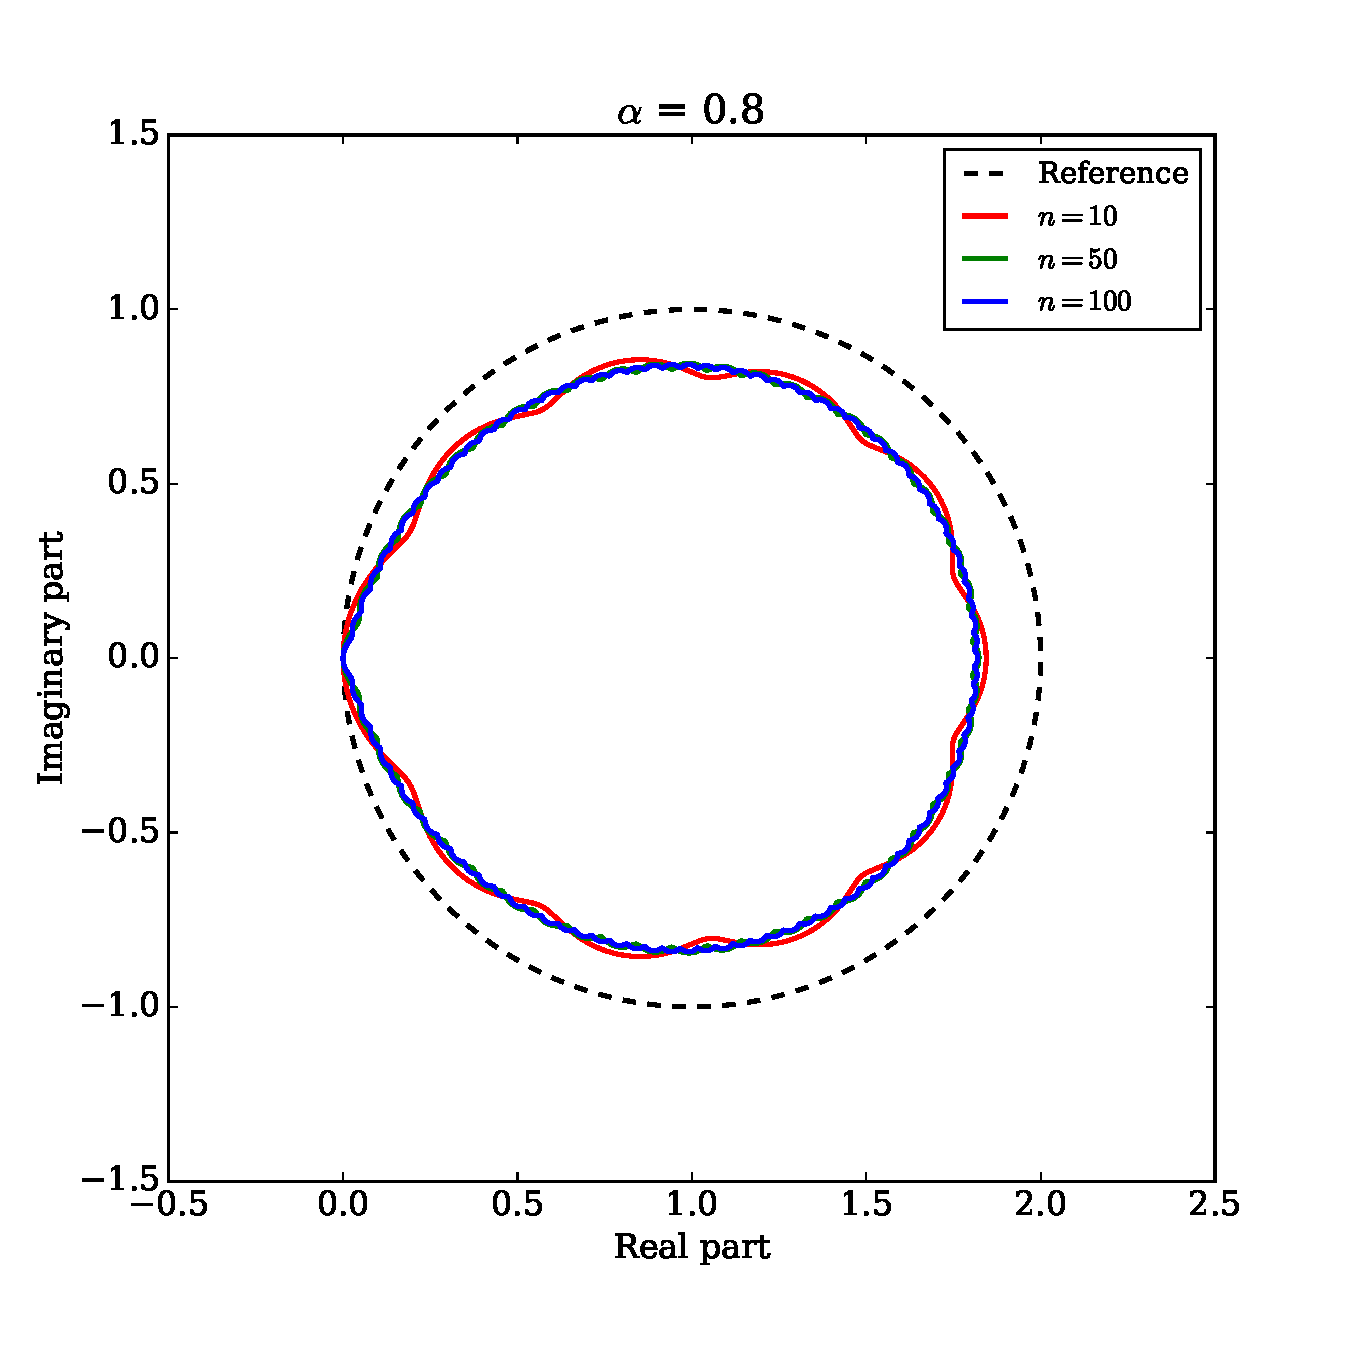
\includegraphics[width=0.45\textwidth]{frac_time/a}
	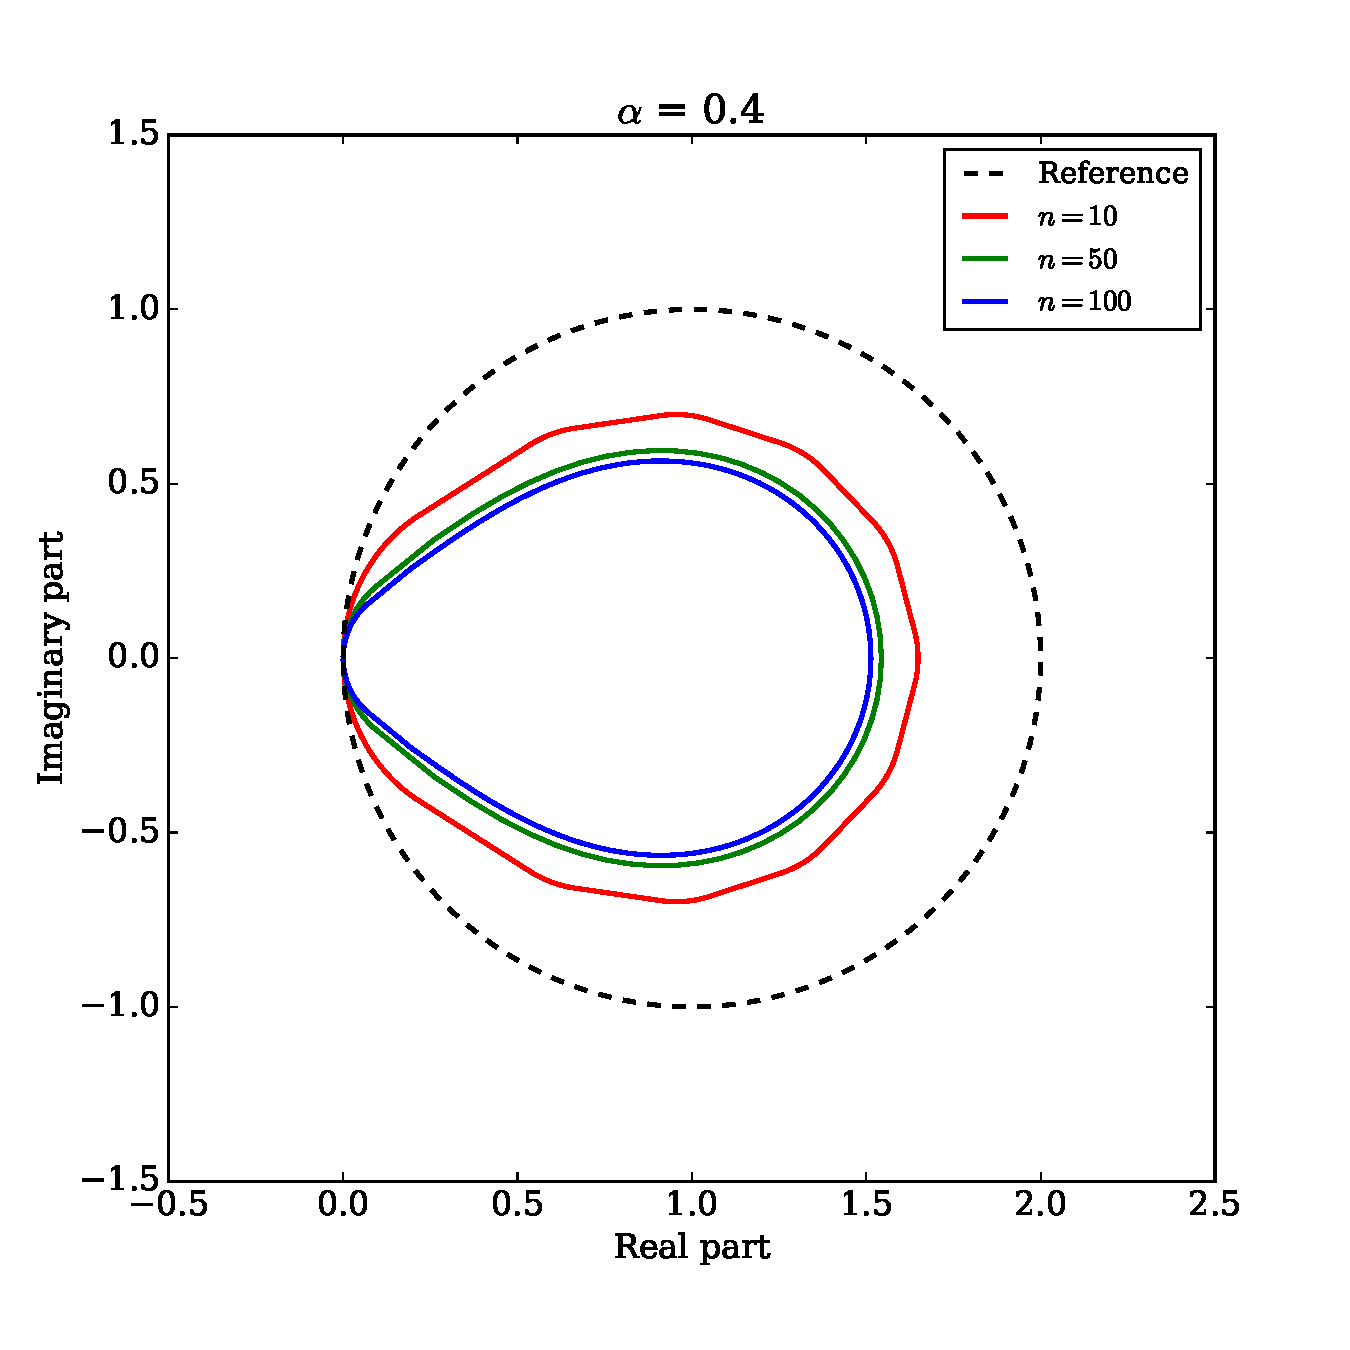
\includegraphics[width=0.45\textwidth]{frac_time/b}
	\bicaption[astability]{左:$\alpha=0.8$,$n=10,50,100$的绝对稳定区域。右:$\alpha=0.4$,$n=10,50,100$的绝对稳定区域。参考:普通导数的向后欧拉方法的稳定区域。}{左:$\alpha=0.8$,$n=10,50,100$的绝对稳定区域。右:$\alpha=0.4$,$n=10,50,100$的绝对稳定区域。参考:普通导数的向后欧拉方法的稳定区域。}{Fig}{Left: Absolute stability zone for $\alpha=0.8$, $n=10,50,100$. Right: Absolute stability zone for $\alpha=0.4$, $n=10,50,100$. Reference: backward Euler for the standard derivative.}
	% \label{astability}
	\end{centering}
\end{figure}


% Notice that, our stability region include the imaginary axis ${\bf Re} (\lambda) = 0$, which is the same case for backward Euler method with standard time derivatives, and thus it has the potential to apply for hyperbolic equations. Although, for hyperbolic problems with standard time derivatives, explicit methods are in general preferred, we shall see that the Caputo time derivatives cause additional constraint in stability, which motivates us to design implicit schemes for \eqref{eq:main}.
请注意,我们的稳定区域包括虚轴${\bf Re}(\lambda)= 0$,这与使用标准时间导数的向后欧拉方法是一样的,因此它可以应用双曲型方程。 虽然,对于标准时间导数的双曲型问题,通常优先选择显式方法,我们将看到Caputo时间导数在稳定性中引起额外的约束,这促使我们为\eqref{eq:main}设计隐式格式。

%\zz{it would be good, if we can add some plots of the stability regions for two different $\alpha$'s.}
\subsection{标量守恒律方程的显示迎风格式}

\subsubsection{一阶格式}
考虑一维的守恒律方程
\begin{equation}\label{eq:cons}
\partial_t^\alpha u+ (f(u))_x=0,
\end{equation}
通量可以分解为
\begin{equation}\label{cond:flux}
f=f^+ + f^- ,\quad (f^+)' \ge 0,\quad (f^-)'\le 0.
\end{equation}
% We make this technique assumption to simplify our analysis. Note that, the flux decomposition is not essential in designing such numerical schemes. The readers may refer to~\citen{wang2003positivity,shu1992numerical} for general discussion on this issue. Without loss of generality, the flux function $f(u)$ might be nonlinear. But obviously, it also includes the linear advection case, when $f=au$.
我们做这个假设来简化我们的分析。注意,在设计这种数值方案时,通量分解不是必不可少的。 读者可以参考\citen{wang2003positivity,shu1992numerical}关于这个问题的一般性讨论。不失一般性,通量函数$f(u)$可能是非线性的。 但是显然,当$f = au$时,它也包括线性对流的情况。

% Again, we assume uniform time step size $\tau$, and denote $t^n=n\tau$, $n=0,1,2,\cdots$. Also, on the computation domain $[a,b]$, we assume uniform spatial grids $x_j= a+j h$, for $j=0,1,\cdots, M$, where the spatial grid size $h=\frac{b-a}{M}$. We denote the numerical approximation of $u\left(x=x_j,t=t^k\right)$ by $U_j^k$. Then, the first order upwind method for the nonlinear conservation law is,
再次,我们假设均匀的时间步长$\tau $,并且记$t ^ n = n\tau $,$ n = 0,1,2,\cdots $。 此外,在计算域$ [a,b] $,我们假设均匀的空间网格$ x_j = a + jh $,对于$ j = 0,1,\cdots,M $,其中空间网格大小$h=\frac{b-a}{M}$。 我们用$ U_j ^ k $表示$u\left(x=x_j,t=t^k\right)$的数值近似值。 然后,非线性守恒律的一阶迎风法格式为,
\begin{equation}\label{firstorder}
D_t^\alpha U^{n+1}_j + \frac{1}{h} \left(f^+ (U_j^n)- f^+(U_{j-1}^n) \right)+\frac{1}{h}\left(f^-(U_{j+1}^n)-f^-(U_j^n)\right) =0.
\end{equation}

如果记
\[
\lambda^{+,n}_j = \frac{a^{+,n}_j  \tau^\alpha \Gamma (2-\alpha)}  {h}, \quad \lambda^{-,n}_j = \frac{a^{-,n}_j  \tau^\alpha \Gamma (2-\alpha)}  {h},
\]
对于在$U^n_{j-1}$和$U^n_{j}$中的$\xi^n_j$以在$U^n_j$ and $U^n_{j+1}$中的$\eta^n_j$,有
\[
a^{+,n}_j=\frac{f^+ (U_j^n)- f^+(U_{j-1}^n)}{U^n_j-U^n_{j-1}}=(f^+)' (\xi^n_j) \ge 0,
\]
\[
a^{-,n}_j=\frac{f^- (U_{j+1}^n)- f^-(U_{j}^n)}{U^n_{j+1}-U^n_{j}}=(f^-)' (\eta^n_j) \le 0,
\]
数值格式可以写为
\begin{equation}\label{reform}
U_j^{n+1}=(\tilde c-\lambda^{+,n}_j +\lambda^{-,n}_j )U_j^{n}+ \lambda^{+,n}_j  U_{j-1}^n -\lambda^{-,n}_j U^n_{j+1}+ \sum_{k=0}^{n-1} c^{n+1}_k U_j^k.
\end{equation}
% Therefore, we propose the following CFL condition for the first order upwind method:
据此,我们给出如下的CFL条件
\begin{equation}\label{CFL}
 \frac{ \tau^\alpha \Gamma (2-\alpha)}  {h} \left( \max |(f^+)'|+\max|(f^-)'| \right)  \le \tilde c.
\end{equation}
% We observe that, the CFL condition essentially agrees with the conservation law with standard time derivatives except that the time step $\tau$ gains an exponent $\alpha$ due to the Caputo derivative.
我们观察到,CFL条件基本上与使用标准时间导数的守恒定律一致,除了时间步长$\tau$获得由Caputo导数产生的指数$\alpha$。

由CFL条件,有
\[
\tilde c-\lambda^{+,n}_j +\lambda^{-,n}_j  \ge 0.
\]
容易得出最大值原理,$\forall n \in \N^+$
\[
\max_j |U^n_j| \le \max_j |U^0_j|. 
\]

% Also, we can show that this method is TVD if the CFL condition \eqref{CFL} is satisfied. Actually, we can rewrite \eqref{reform} as
也可以证明在CFL条件\eqref{CFL}下方法是TVD的。事实上,可以将\eqref{reform}写作
\begin{equation}
U_j^{n+1}=\tilde c U_j^{n}-\delta f^+(U^n_j) +\delta f^+(U^n_j)  + \delta f^+(U^n_{j-1})-\delta f^+(U^n_{j+1})+ \sum_{k=0}^{n-1} c^{n+1}_k U_j^k,
\end{equation}
其中$\delta =\frac{  \tau^\alpha\Gamma (2-\alpha)}  {h }$。考虑满足同一个差分方程的另外一个解$V^n_j$,
\begin{equation}
V_j^{n+1}=\tilde c V_j^{n}-\delta f^+(V^n_j) +\delta f^+(V^n_j)  + \delta f^+(V^n_{j-1})-\delta f^+(V^n_{j+1})+ \sum_{k=0}^{n-1} c^{n+1}_k V_j^k.
\end{equation}
两式相减
\begin{align*}
U_j^{n+1}-V_j^{n+1} &=\tilde c \left( U_j^{n}-V_j^{n}\right) -\delta \left(f^+(U^n_j)-f^+(V^n_j) \right) +\delta \left(f^-(U^n_j)-f^-(V^n_j) \right) \\
& +\delta \left(f^+(U^n_{j-1})-f^+(V^n_{j-1}) \right) - \delta \left(f^-(U^n_{j+1})-f^-(V^n_{j+1}) \right) + \sum_{k=0}^{n-1} c^{n+1}_k \left( U_j^k- V_j^k \right).
\end{align*}
根据均值理论
\begin{align*}
U_j^{n+1}-V_j^{n+1} &=\left(\tilde c -\delta (f^+)'(\xi_j^+) +\delta (f^-)'(\xi_j^-)\right)\left( U_j^{n}-V_j^{n}\right)+\delta   (f^+)'(\xi_{j-1}^+) \left( U_{j-1}^{n}-V_{j-1}^{n}\right) \\
& - \delta   (f^-)'(\xi_{j+1}^-) \left( U_{j+1}^{n}-V_{j+1}^{n}\right) + \sum_{k=0}^{n-1} c^{n+1}_k \left( U_j^k- V_j^k \right),
\end{align*}
其中$\xi_j^+$和$\xi_j^-$为$U^{n}_j$和$V^{n}_j$之间的数。
注意当满足CFL条件\eqref{CFL}时
\[
\tilde c -\delta (f^+)'(\xi_j^+) +\delta (f^-)'(\xi_j^-) \ge0,
\]
根据三角不等式
\begin{align*}
\left| U_j^{n+1}-V_j^{n+1} \right| &=\left(\tilde c -\delta (f^+)'(\xi_j^+) +\delta (f^-)'(\xi_j^-)\right)\left| U_j^{n}-V_j^{n}\right|+\delta   (f^+)'(\xi_{j-1}^+) \left| U_{j-1}^{n}-V_{j-1}^{n}\right| \\
& - \delta   (f^-)'(\xi_{j+1}^-) \left| U_{j+1}^{n}-V_{j+1}^{n}\right| + \sum_{k=0}^{n-1} c^{n+1}_k \left| U_j^k- V_j^k \right|.
\end{align*}
对$j$求和
\[
\sum_j \left|U^{n+1}_j-V^{n+1}_{j} \right|  \le  \sum_{k=0}^{n} c^{n+1}_k   \sum_j  \left| U_j^k- V_{j}^k\right|.
\]
这里,通量项都消掉了,由归纳法,
\[
 \|U^n-V^n\|_{\ell^1} \le \|U^0-V^0\|_{\ell^1},
 \] 
即,我们证明了如下定理
\begin{thm}
当满足CFL条件\eqref{CFL}时,方程\eqref{eq:main}的一阶迎风格式\eqref{firstorder}是$\ell^1$递减的。
\end{thm}

作为一个直接的推论,如果取$V^n_j$为$U^{n}_{j+1}$,得到对于$n\in \N^+$,
\[
\mbox{TV}\left[U^n\right] \le \mbox{TV}\left[U^0\right]  ,
 \]
 其中$\mbox{TV}\left[U^n\right]= \sum_j | U^n_{j+1}-U^n_j | $。也就是
 \begin{cor}
 当满足CFL条件\eqref{CFL}时,方程\eqref{eq:main}的一阶迎风格式\eqref{firstorder}是TVD的。
 \end{cor}


%Clearly, the $\ell^1$ contacting property of the method implies that the method is TVD.

\subsubsection{MUSCL格式}

% To construct a second order method in space, the positive and negative fluxes can be approximated by the piecewise linear function,
为了构造一个空间方向二阶的格式,正负通量可用分段线性函数逼近
\[
f^{\pm,n}(x)=f^{\pm,n}_j + s^{\pm,n}_j (x-x_j),\quad x_{j-\frac 1 2}< x <x_{j+\frac 1 2},
 \] 
其中记$f^{\pm,n}_j=f^{\pm,n}(U^n_j)$。斜率函数由通量限制器定义
\[
s^{\pm,n}_j  = \frac{f^{\pm,n}_j-f^{\pm,n}_{j-1}}{h} \phi^0 \left( \frac{f^{\pm,n}_{j+1}-f^{\pm,n}_{j}}{f^{\pm,n}_j-f^{\pm,n}_{j-1}}  \right).
\]
本章中我们仅考虑minmod限制器
\[
\phi^0 (\theta) = \max (0, \min(1,\theta)),
\]
或Van Leer限制器
\[
\phi^0(\theta)= \frac{|\theta|+\theta}{1+\theta}.
\]
% Note that, both limiters are symmetric, i.e., $a \phi^0(b/a) = b \phi^0 (a/b)$. Consequently, the second-order flux splitting method is given by
注意,这两种限制器都是对称的,即$a \phi^0(b/a) = b \phi^0 (a/b)$。二阶通量分裂格式为
\[
D_t^\alpha U^{n+1}_j + \frac{1}{h} \left(f^{+,n} (x_{j+\frac 1 2}-)- f^{+,n}(x_{j-\frac 1 2}-) \right)+\frac{1}{h}\left(f^{-,n} (x_{j+\frac 1 2}+)-f^{-,n} (x_{j-\frac 1 2}+)\right) =0.
\]
或等价的
\[
D_t^\alpha U^{n+1}_j + \psi_j^{+,n}\frac{f^{+,n}_j-f^{+,n}_{j-1}}{h} + \psi^{-,n}_j \frac{f^{-,n}_{j+1}-f^{-,n}_{j}}{h}=0.
\]
系数
\[
\psi_j^{+,n}=1 + \frac 1 2 \phi^0 \left(\frac{f^{+,n}_{j+1}-f^{+,n}_{j}}{f^{+,n}_j-f^{+,n}_{j-1}} \right) - \frac 1 2 \phi^0   \left(\frac{f^{+,n}_{j-1}-f^{+,n}_{j-2}}{f^{+,n}_j-f^{+,n}_{j-1}} \right),
\]
\[
\psi_j^{-,n}=1 + \frac 1 2 \phi^0 \left(\frac{f^{-,n}_{j+2}-f^{-,n}_{j+1}}{f^{-,n}_{j+1}-f^{-,n}_{j}} \right) - \frac 1 2 \phi^0   \left(\frac{f^{-,n}_{j}-f^{-,n}_{j-1}}{f^{-,n}_{j+1}-f^{-,n}_{j}} \right).
\]
% Again, one can apply the mean value theorem for $f^+$ and $f^-$, and the second order flux splitting scheme for the nonlinear conservation law problem can still be reformulated in the form of \eqref{reform}, with
同样的,可以对于$f^+$和$f^-$应用均值理论。非线性守恒律的二阶通量分裂格式可以改写为\eqref{reform}的形式,其中
\[
a^{+,n}_j=\psi_j^{+,n}(f^+)' (\xi^n_j),\quad a^{-,n}_j=\psi_j^{-,n}(f^-)' (\eta^n_j) .
\]

因为限制器满足
\[
0 \le \frac{\phi^0 (\theta)}{\theta} \le 2,\quad 0 \le \phi^0(\theta) \le 2,
\]
所以系数$\psi_j^{\pm,n} \in [0,2]$,这表明$\pm a^{\pm,n}_j$是非负的。同理,可以提出如下CFL条件
\begin{equation}\label{CFL2}
 2 \frac{ \tau^\alpha \Gamma (2-\alpha)}  {h} \left( \max |(f^+)'|+\max|(f^-)'| \right)  \le \tilde c.
\end{equation}
% Clearly, with the above condition, the coefficients on the right hand side of the form \eqref{reform} are all nonnegative. Therefore, we can conclude conditional TVD properties and stability properties by the argument similar to the first order cases.
显然,在上述条件下,\eqref{reform}右侧的系数都是非负的。 因此,我们可以通过类似于一阶情况的论证来得出TVD和稳定性。

% We observe that, for explicit methods of conservation laws, although the stability constraint only changes to $\tau^\alpha = O(h)$ due to the Caputo derivative, in practice, it makes these methods infeasible. For example, when $\alpha= \frac{1}{2}$, this constraint is already as restricted as explicit methods for parabolic equations. And, when $\alpha \rightarrow 0$, the choice of time steps suffers severely from the CFL conditions. 
我们观察到,对于显式的格式,尽管由于Caputo导数,稳定性约束只改变为$\tau^\alpha = O(h)$,但在实践中,这使得这些方法不可行。 例如,当$\alpha = \frac{1}{2}$时,该约束已经像抛物型方程的显式方法一样受到限制。而当$ \alpha \rightarrow 0 $时,时间步长的选择由CFL条件可以知是非常非常小的。
%Next, if we denote $U^n=(U_0^n,U_1^n,\cdots,U_M^n)$ and denote the (discrete) total variance
%\[
%\mbox{TV}(U^n)=\sum_{j=1}^M |U^n_j-U^n_{j-1}|,
%\]
%Then, by direct calculation, if the CFL condition is satisfied
%\begin{align*}
%\mbox{TV}(U^{n+1})&=\sum_{j=1}^M |U^{n+1}_j-U^{n+1}_{j-1}| \\
%& =\sum_{j=1}^M |(c_n-\lambda) (U^n_j-U^n_{j-1})+\lambda(U^n_{j+1}-U^n_j)+\sum_{k=0}^{n-1}c_k (U^k_j-U^k_{j-1}) | \\
%& \le (c_n-\lambda)\sum_{j=1}^n|U^n_j-U^n_{j-1}| + \lambda\sum_{j=1}^n|U^n_{j+1}-U^n_{j}| \\
%&\quad +\sum_{k=0}^{n-1}c_k \sum_{j=1}^n|U^n_j-U^n_{j-1}|.
%\end{align*}
%Therefore, we immediately conclude that, $\forall n \in \N^+$,
%\[
%\mbox{TV}(U^n) \le \mbox{TV}(U^0).
%\]
%Hence, we conclude the upwind method for the fractional time derivative advection equation is TV-stable.
%
%We remark that when $v<0$, all the analysis and results can be carried out in the same way.
\subsection{标量守恒律方程的隐式格式}
\subsubsection{稳定性分析}
% As we see in the previous section, albeit we are able to derive modified CFL condition for the scalar conservation law,  the stability constraint implies that the time step $\Delta t$ is a higher order small quantity of the spatial size $\Delta x$. Therefore, we are motivated to analyze the implicit upwind scheme for equation  \eqref{eq:cons} with the flux function $f$ satisfies the condition \eqref{cond:flux}, which is given by
正如我们在上一节中所看到的,尽管我们能够得到标量守恒定律的修正CFL条件,但稳定性约束意味着时间步长$\Delta t$是空间网格大小$\Delta x $的较高阶量级。 因此,我们需要分析方程\eqref{eq:cons}的隐式迎风方案,其中通量函数$f$满足条件\eqref{cond:flux},由
\begin{equation}\label{imfirst}
D_t^\alpha U^{n+1}_j + \frac{1}{h} \left(f^+ (U_{j-1}^{n+1})- f^+(U_{j-2}^{n+1}) \right)+\frac{1}{h}\left(f^-(U_{j+1}^{n+1})-f^-(U_j^{n+1})\right) =0.
\end{equation}


我们引入类似的记号来重写格式
\[
\lambda^{+,n}_j = \frac{a^{+,n}_j  \tau^\alpha \Gamma (2-\alpha)}  {h}, \quad \lambda^{-,n}_j = \frac{a^{-,n}_j  \tau^\alpha \Gamma (2-\alpha)}  {h},
\]
对于某些$U^{n+1}_{j-1}$和$U^{n+1}_{j}$之间的$\xi^{n+1}_j$,$U^{n+1}_j$和$U^{n+1}_{j+1}$之间的某些$\eta^{n+1}_j$,有
\[
a^{+,n+1}_j=\frac{f^+ (U_j^{n+1})- f^+(U_{j-1}^{n+1})}{U^{n+1}_j-U^{n+1}_{j-1}}=(f^+)' (\xi^{n+1}_j) \ge 0,
\]
\[
a^{-,n+1}_j=\frac{f^- (U_{j+1}^{n+1})- f^-(U_{j}^{n+1})}{U^{n+1}_{j+1}-U^{n+1}_{j}}=(f^-)' (\eta^{n+1}_j) \le 0,
\]
格式重写为
\begin{equation}\label{reform2}
U_j^{n+1}-\sum_{k=0}^{n} c^{n+1}_k U_j^k= -\lambda^{+,n+1}_j \left(U^{n+1}_j-U^{n+1}_{j-1}\right) -  \lambda^{-,n+1}_j \left(U^{n+1}_{j+1}-U^{n+1}_{j}\right).
\end{equation}

现在我们来证明下述定理
\begin{thm}
守恒律方程\eqref{eq:main} 的隐式迎风格式\eqref{imfirst}为无条件$\ell^1$递减的。 
\end{thm}
\begin{proof}
重写\eqref{reform2}
\begin{equation}\label{reform3}
U_j^{n+1}-\sum_{k=0}^{n} c^{n+1}_k U_j^k= -\delta \left(f^+ (U_{j-1}^{n+1})- f^+(U_{j-2}^{n+1})\right) -\delta \left(f^-(U_{j+1}^{n+1})-f^-(U_j^{n+1})\right) .
\end{equation}
注意$\delta=\frac{\tau^\alpha}{h}$。设${V^n_j}$是同一个方程相同数值格式的解,
\begin{equation}\label{reform4}
V_j^{n+1}-\sum_{k=0}^{n} c^{n+1}_k V_j^k= -\delta \left(f^+ (V_{j-1}^{n+1})- f^+(V_{j-2}^{n+1})\right) -\delta \left(f^-(V_{j+1}^{n+1})-f^-(V_j^{n+1})\right) .
\end{equation}

%Firstly, we aim to show that the implicit upwind scheme is TV-stable. we shift the spatial index $j$ to $j-1$, and get
%\[
%U_{j-1}^{n+1}-\sum_{k=0}^{n} c^{n+1}_k U_{j-1}^k= -\lambda^{+,n}_{j-1} \left(U^{n+1}_{j-1}-U^{n+1}_{j-2}\right) -  \lambda^{-,n}_{j-1} \left(U^{n+1}_{j}-U^{n+1}_{j-1}\right).
%\]

两式相减,应用均值理论
\begin{multline*}
 U_j^{n+1} -V_{j}^{n+1} +\delta (f^+)'(\xi_j^+) \left(U^{n+1}_j-V^{n+1}_{j}\right) -  \delta (f^-)'(\xi_j^-)  \left(U^{n+1}_{j}-V^{n+1}_{j}\right) = \\
 \sum_{k=0}^{n} c^{n+1}_k \left( U_j^k- V_{j}^k\right) -  \delta (f^-)'(\xi_{j-1}^-)  \left(U^{n+1}_{j+1}-V^{n+1}_{j+1}\right)  -\delta (f^+)'(\xi_{j-1}^+)  \left(U^{n+1}_{j-1}-V^{n+1}_{j-1}\right),
 \end{multline*}
$\xi_j^+$和$\xi_j^-$是$U^{n+1}_j$和$V^{n+1}_j$之间的数。
 
 
% Multiply each side by $\mbox{Sgn} \left(U^{n+1}_j-U^{n+1}_{j-1}\right) $,  and sum over $j$, we get
% \begin{align*}
% \mbox{L.H.S.} & = \sum_j \left|U^{n+1}_j-U^{n+1}_{j-1} \right| + \sum_j  \lambda^{+,n}_j \left(U^{n+1}_j-U^{n+1}_{j-1}\right) -  \sum_j \lambda^{-,n}_{j-1} \left(U^{n+1}_{j}-U^{n+1}_{j-1}\right)  \\
% & =  \sum_j \left|U^{n+1}_j-U^{n+1}_{j-1} \right| + \sum_j \left( \left| \lambda^{+,n}_j \left(U^{n+1}_j-U^{n+1}_{j-1}\right)\right| +  \left| \lambda^{-,n}_{j-1} \left(U^{n+1}_{j}-U^{n+1}_{j-1}\right) \right| \right) \\
% &= \sum_j \left|U^{n+1}_j-U^{n+1}_{j-1} \right| \\
%& \quad +  \sum_j  \frac{\tau^\alpha}{h C_\alpha} \left[\left| f^+\left( U^{n+1}_j\right)- f^+\left( U^{n+1}_{j-1}\right) \right|+  \left| f^-\left( U^{n+1}_j\right)- f^+\left( U^{n+1}_{j-1}\right) \right|\right].
% \end{align*}
% For the right hand side, by triangle inequality, we obtain,
%   \begin{align*}
%    \mbox{R.H.S.} & \le \sum_j \sum_{k=0}^{n} c^{n+1}_k \left| U_j^k- U_{j-1}^k\right| +\sum_j \left( \left| \lambda^{+,n}_j \left(U^{n+1}_{j-1}-U^{n+1}_{j-2}\right)\right| +  \left| \lambda^{-,n}_{j-1} \left(U^{n+1}_{j+1}-U^{n+1}_{j}\right) \right| \right)   \\
% &=  \sum_j \sum_{k=0}^{n} c^{n+1}_k \left| U_j^k- U_{j-1}^k\right| \\
%& \quad +  \sum_j  \frac{\tau^\alpha}{h C_\alpha} \left[\left| f^+\left( U^{n+1}_j\right)- f^+\left( U^{n+1}_{j-1}\right) \right|+  \left| f^-\left( U^{n+1}_j\right)- f^+\left( U^{n+1}_{j-1}\right) \right|\right].
%    \end{align*}
    
两边同乘$\mbox{Sgn} \left(U^{n+1}_j-V^{n+1}_{j}\right) $,对$j$求和,得到
 \begin{align*}
 \mbox{L.H.S.} & = \sum_j \left|U^{n+1}_j-V^{n+1}_{j} \right| + \sum_j  \delta (f^+)'(\xi_j^+)  \left|U^{n+1}_j-V^{n+1}_{j}\right| -  \sum_j \delta (f^-)'(\xi_j^-)  \left(U^{n+1}_{j}-V^{n+1}_{j}\right)  \\
 & =  \sum_j \left|U^{n+1}_j-V^{n+1}_{j} \right| + \delta \sum_j \left( \left|\delta (f^+)'(\xi_j^+)  \left(U^{n+1}_j-V^{n+1}_{j}\right)\right| +  \left| (f^-)'(\xi_j^-)  \left(U^{n+1}_{j}-V^{n+1}_{j}\right) \right| \right) \\
 &= \sum_j \left|U^{n+1}_j-V^{n+1}_{j} \right|  +  \delta \sum_j   \left[\left| f^+\left( U^{n+1}_j\right)- f^+\left( V^{n+1}_{j}\right) \right|+  \left| f^-\left( U^{n+1}_j\right)- f^+\left( V^{n+1}_{j}\right) \right|\right].
 \end{align*}
右端由三角不等式,
   \begin{align*}
    \mbox{R.H.S.} & \le \sum_j \sum_{k=0}^{n} c^{n+1}_k \left| U_j^k- V_{j}^k\right| +\delta \sum_j \left( \left|(f^+)'(\xi_{j-1}^+)  \left(U^{n+1}_{j-1}-V^{n+1}_{j-1}\right)\right| +  \left| (f^-)'(\xi_{j+1}^-)  \left(U^{n+1}_{j+1}-V^{n+1}_{j+1}\right) \right| \right)   \\
 &=  \sum_j \sum_{k=0}^{n} c^{n+1}_k \left| U_j^k- V_{j}^k\right| +  \delta \sum_j  \left[\left| f^+\left( U^{n+1}_j\right)- f^+\left( V^{n+1}_{j}\right) \right|+  \left| f^-\left( U^{n+1}_j\right)- f^+\left( V^{n+1}_{j}\right) \right|\right].
    \end{align*}
    
得到
\[
\sum_j \left|U^{n+1}_j-V^{n+1}_{j} \right|  \le \sum_j \sum_{k=0}^{n} c^{n+1}_k \left| U_j^k- V_{j}^k\right|.
\]
根据归纳法,
\[
 \|U^n-V^n\|_{\ell^1} \le \|U^0-V^0\|_{\ell^1},
 \] 
即隐式迎风格式是$\ell^1$递减的。
\end{proof}
类似于之前的情况,我们有
\begin{cor} 
守恒律方程\eqref{eq:main} 的隐式迎风格式\eqref{imfirst} 是无条件VD的。
\end{cor}

\subsubsection{能量估计和熵解}
% To further investigate the numerical dissipation introduced when approximating the Caputo derivative, we apply the following energy method, and show that the implicit upwind  method is unconditionally $l^2$ stable for the linear advection equation, i.e. $f=au$. For simplicity, we take $a>0$, then the right hand side of  \eqref{reform2} reduces to
为了进一步研究近似Caputo导数时引入的数值耗散,我们应用以下能量法,并且证明隐式迎风方法对于线性对流方程,即$f = au$无条件地为$l ^ 2$稳定。 为了简单起见,我们取$ a> 0 $,那么右边的\eqref{reform2}化为
\[
\mbox{R.H.S.} = -\lambda \left(U^{n+1}_j-U^{n+1}_{j-1}\right) ,
\]
其中$\lambda= a \tau^ \alpha\Gamma(2-\alpha)/ h$。


\eqref{reform2}两边乘$U_j^{n+1}$,对$j$求和,得到
\begin{align*}
\mbox{L.H.S.} &=\sum_j  U_j^{n+1} \left( U_j^{n+1}-\sum_{k=0}^{n} c^{n+1}_k U_j^k \right) \\
&= \sum_j \sum_{k=0}^{n} c^{n+1}_k  \left[ \left( U_j^{n+1} \right)^2 -U_j^{n+1}U_j^{k}  \right] \\
&= \frac{1}{2} \sum_j \sum_{k=0}^{n}  c^{n+1}_k   \left[ \left( U_j^{n+1} \right)^2 + \left( U_j^{n+1}-U_j^{k} \right)^2 -  \left( U_j^{k} \right)^2  \right] \\
& = \frac{1}{2}  \sum_j \left( U_j^{n+1} \right)^2 + \frac{1}{2} \sum_j \sum_{k=0}^{n} c^{n+1}_k \left( U_j^{n+1}-U_j^{k} \right)^2 -  \frac{1}{2} \sum_j \sum_{k=0}^{n}  c^{n+1}_k \left( U_j^{k} \right)^2  \\
& =\frac{1}{2} \| U^{n+1} \|_{l^2}^2 - \frac 1 2 \sum_{k=0}^{n}  c^{n+1}_k \|U^k \|_{l^2}^2 + \frac{1}{2} \sum_j \sum_{k=0}^{n} c^{n+1}_k \left( U_j^{n+1}-U_j^{k} \right)^2.
\end{align*}
和
\begin{align*}
\mbox{R.H.S.} &=\sum_j  -\lambda  U_j^{n+1} \left(U^{n+1}_j-U^{n+1}_{j-1}\right)  \\
& = -\frac \lambda 2 \sum_j \left[ \left( U_j^{n+1}\right)^2 -2 U_j^{n+1} U_{j-1}^{n+1}+\left( U_{j-1}^{n+1}\right)^2 \right] \\
& = -\frac \lambda 2 \sum_j \left(  U_j^{n+1} - U_{j-1}^{n+1} \right)^2.
\end{align*}

因此得到
\[
\| U^{n+1} \|_{l^2}^2 + \sum_j \sum_{k=0}^{n} c^{n+1}_k \left( U_j^{n+1}-U_j^{k} \right)^2+ \lambda  \sum_j \left(  U_j^{n+1} - U_{j-1}^{n+1} \right)^2 = \sum_{k=0}^{n}  c^{n+1}_k \|U^k \|_{l^2}^2.
\]
根据归纳法,可以容易的证明对于$n\in \N^+$, $\| U^{n} \|_{l^2}^2  \le   \| U^{0} \|_{l^2}^2 $,所以我们有如下估计,
\[
 \| U^{n} \|_{l^2}^2 + \sum_j  \sum_{k=0}^{n-1} c^{n}_k \left( U_j^{n}-U_j^{k} \right)^2+ \lambda \sum_j  \left(  U_j^{n} - U_{j-1}^{n} \right)^2 \le   \| U^{0} \|_{l^2}^2 .
\]
% We remark that the second term of the left hand side corresponds to the damping effect of the fractional time derivative, and the third term of the left hand side corresponds to the numerical dissipation by the upwind method.
左边的第二项对应于分数时间导数的阻尼效应,左侧的第三项对应于逆风方法的数值耗散。

%\subsubsection{Entropy}

% At last, we want to verify that, the implicit upwind method also satisfies the entropy condition for the linear advection equation. Assume that $\eta(u)$ is a convex entropy function and $\psi(u)$ is its entropy flux function. For the linear advection equation, we have clearly $\psi(u)=a \eta(u)$. Without loss of generality, we take $a>0$, and we rewrite the implicit upwind scheme in the following way,
最后,我们要验证,隐式迎风方法也满足线性对流方程的熵条件。假设$ \eta(u)$是一个凸熵函数,$ \psi(u)$是其熵通量函数。 对于线性对流方程,我们有$ \psi(u)= a \eta(u)$。 在不失一般性的情况下,我们取$ a> 0 $,并以下列方式重写隐式迎风方格式:
\[
U_j^{n+1}  +\lambda U^{n+1}_j=\sum_{k=0}^{n} c^{n+1}_k U_j^k  +\lambda U^{n+1}_{j-1},
\]
其中$\lambda= a \tau^ \alpha/ (h C_\alpha)$。两边同除$1+\lambda$,
\[
U_j^{n+1}=\sum_{k=0}^{n} \frac{c^{n+1}_k}{1+\lambda} U_j^k  +\frac{\lambda}{1+\lambda} U^{n+1}_{j-1}.
\]
显然,右端为一个凸组合
\[
\sum_{k=0}^{n} c^{n+1}_k + \lambda = 1+ \lambda, \quad c_k^{n+1}>0.
\]
熵函数的凸性表明
\[
\eta \left( U_j^{n+1} \right)=\eta \left( \sum_{k=0}^{n} \frac{c^{n+1}_k}{1+\lambda} U_j^k  +\frac{\lambda}{1+\lambda} U^{n+1}_{j-1} \right) \le \sum_{k=0}^{n} \frac{c^{n+1}_k}{1+\lambda}  \eta \left( U_j^k \right) +\frac{\lambda}{1+\lambda}\eta \left( U^{n+1}_{j-1} \right).
\]
对$j$求和并记$\eta(U^n)= \sum_j \eta(U^N_j)$,得到
\[
\eta \left( U^{n+1} \right) \le \sum_{k=0}^{n} {c^{n+1}_k} \eta \left( U^k \right). 
\]
根据归纳法
\[
\eta \left( U^{n+1} \right) \le  \eta \left( U^0 \right),
\]
说明离散的熵是不减的。

% For general conservation laws with Caputo derivatives, it is possible to show similar results. However, the analytical aspect of entropy solutions to conservation law with the Caputo derivatives is not completely understood yet. Therefore, we would leave the related numerical analysis as one of the possible future directions. But in this work, we would instead conduct various numerical tests.
对于具有Caputo导数的一般的守恒律,可以证明类似的结果。 然而,Caputo导数的熵解与守恒定律的分析方面尚未完全了解。 因此,我们将把相关的数值分析作为未来可能的方向之一。 但在这项工作中,我们将进行各种数值测试。
%%%%%%%%%%%%%%%%%%%%%%%%%%



\section{数值例子}
%\citen{Agrawal:2002hvba}, \citen{Néel:2007jgba}, \citen{Paradisi:2001beba}, \citen{Xu:2007eaba}, \citen{Xu:2013jjba}, \citen{Zhao:2015gfba}
\subsection{显式格式的例子}
% In this section, we will give numerical examples of our first and second order explicit schemes for scalar advection equations.
首先我们给出标量对流方程的一阶、二阶显式格式的例子,考虑如下方程:
% First, we consider the following advection equation:
\begin{equation}
\partial_t^\alpha u+\partial_x u = 0,
\end{equation}
及不连续的初值
\begin{equation}
u(x, 0) = \begin{cases}
2, \quad \mbox{if } x < 0, \\
1, \quad \mbox{if } x \geq 0.
\end{cases}
\end{equation}

\subsubsection{一阶格式的收敛性和稳定性测试}	
% For the convergence tests, we will fix $\Delta t = 0.0001$ and compute the solution at time $T = 0.2$. The reference solution is obtained by using a fine mesh with $\Delta x = 0.001$ and $\Delta t = 0.0001$. The measure of error here we use is the $\ell^1$ error which is:
收敛性测试中,我们固定$\Delta t = 0.0001$并计算在$T = 0.2$时的解。参考解是用非常细的网格$\Delta x = 0.001$盒$\Delta t = 0.0001$得到的。误差使用$\ell^1$来衡量:
\begin{equation}
\mathrm{error} = \|u(x_j, T) - u_{\mathrm{ref}}\|_{\ell^1}.
\end{equation}
% To make a comparison, we will test with $\alpha = 0.8$ and $\alpha = 0.9$ respectively. %\zz{include $\Delta t$ information.}
% The result is shown in Figure \ref{fig_conv_ex1}:
作为比较,分别令$\alpha = 0.8$及$\alpha = 0.9$。结果显示在图\ref{fig_conv_ex1}中:
\begin{figure}[htbp]
	\centering
	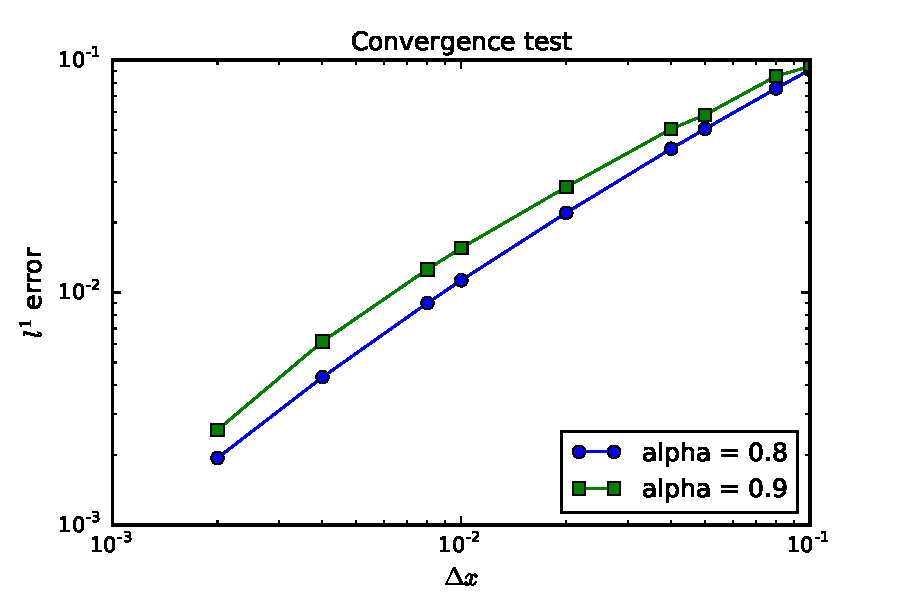
\includegraphics[width=0.8\textwidth]{frac_time/conv_ex}
	\bicaption[fig_conv_ex1]{收敛性测试表明为$\Delta x$的一阶收敛。}{收敛性测试表明为$\Delta x$的一阶收敛。}{Fig}{Convergence test shows it is a first order scheme in $\Delta x$.}
	% \label{fig_conv_ex1}
\end{figure}
从log-log图中可以看出这是一个一阶格式。

% For the stability tests we will fix $\Delta x = 0.01$ and let $\Delta t$ increase from fine to coarse, we show the empirical critical value of $\Delta t$ which makes our scheme diverges as shown in the lower row of Figure \ref{sta_ex1}, which is compared with results computed with the largest $\Delta t$ satisfying the proposed CFL condition \eqref{CFL}.  We observe that, the stability conditions we derived are basically sharp.
对于稳定性测试,我们将固定$ \Delta x = 0.01 $,并且让$ \Delta t $从小到大增加,我们显示出使得我们的格式发散的$ \Delta t $的临界值,在图\ref{sta_ex1}中。该结果与满足CFL条件\eqref{CFL}的最大$ \Delta t $计算结果进行比较。 我们观察到,我们得出的稳定性条件基本上是很准确的。

% We observe that the constriction on $\Delta t$ is severely strict when using explicit methods, which makes the computation really time consuming. In particular, the stability condition is extremely restricted as $\alpha \rightarrow 0$, and makes the implementation impractical.
我们观察到,当使用显式方法时,对$ \Delta t $的约束是非常严格的,这使得计算非常耗时。 特别地,稳定性条件非常受限于$ \alpha \rightarrow 0 $,在应用中非常受限。
%\zz{you should include the threshold $\Delta t$ from the CFL condition.}

\begin{figure}
	\centering
	\subfigure{
		\begin{minipage}[b]{0.305\textwidth}
			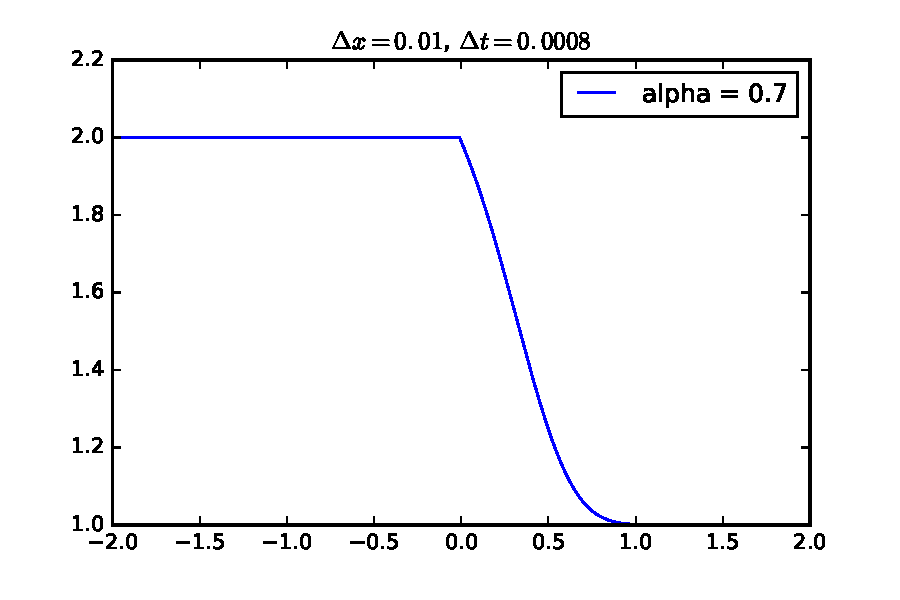
\includegraphics[width=1\textwidth]{frac_time/sta_1} \\
			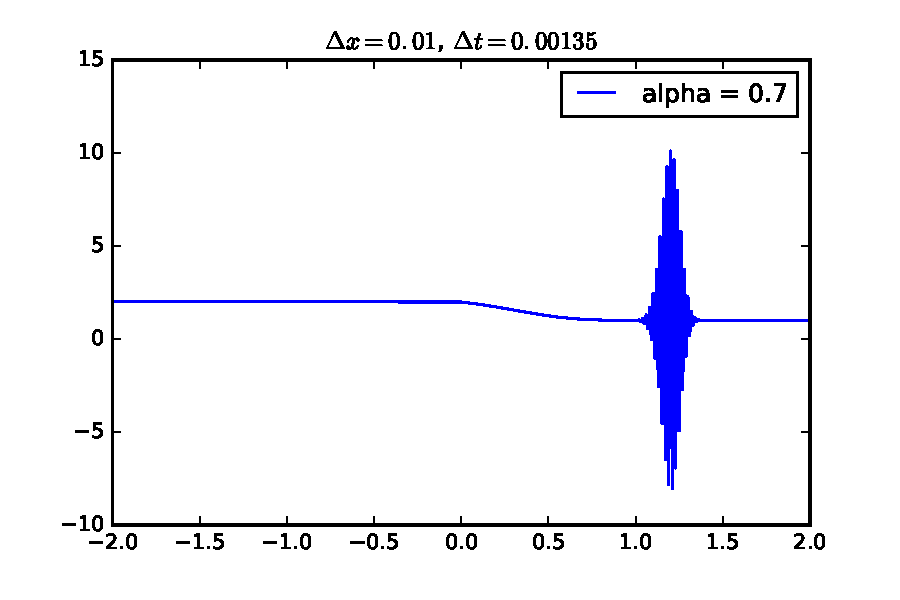
\includegraphics[width=1\textwidth]{frac_time/usta_1}
		\end{minipage}
	}
	\subfigure{
		\begin{minipage}[b]{0.305\textwidth}
			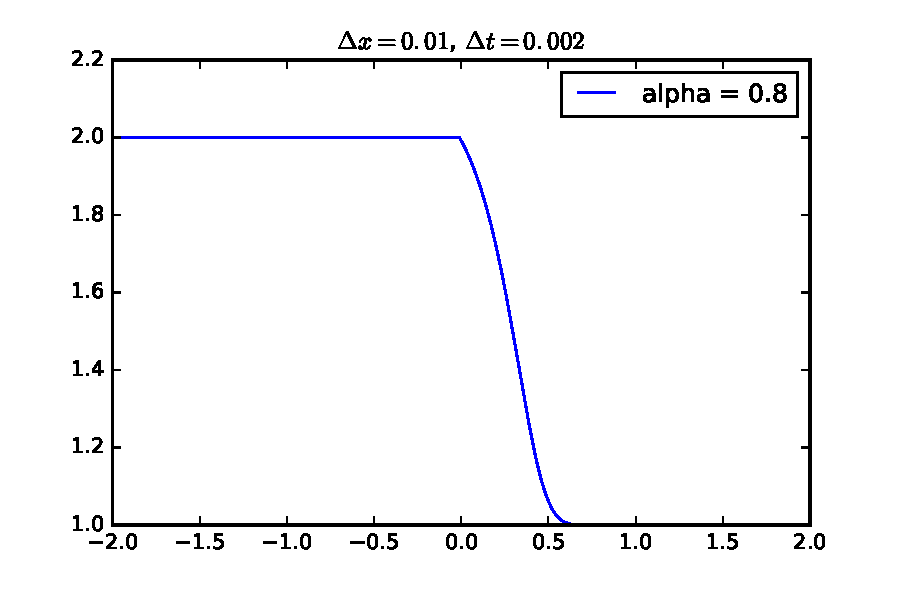
\includegraphics[width=1\textwidth]{frac_time/sta_2} \\
			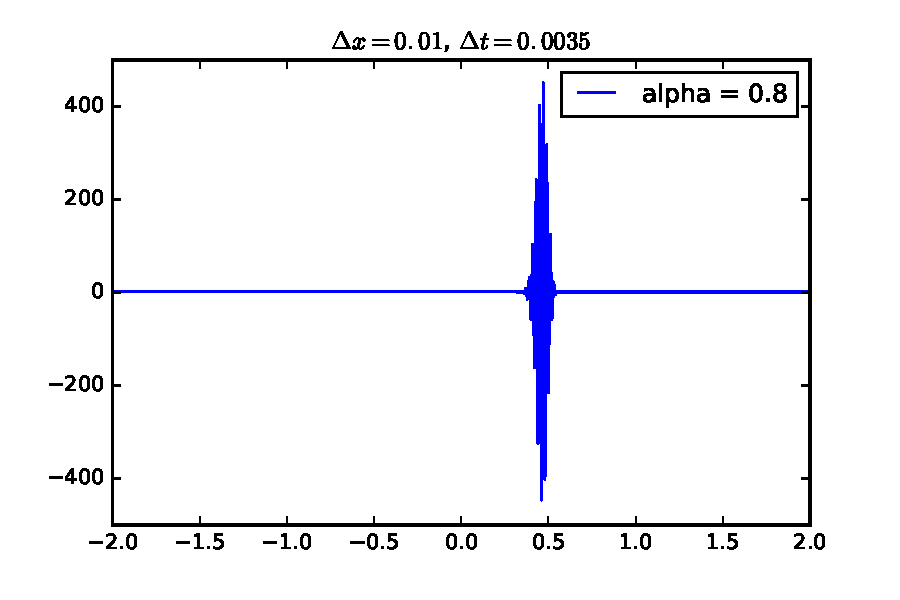
\includegraphics[width=1\textwidth]{frac_time/usta_2}
		\end{minipage}
	}
	\subfigure{
		\begin{minipage}[b]{0.305\textwidth}
			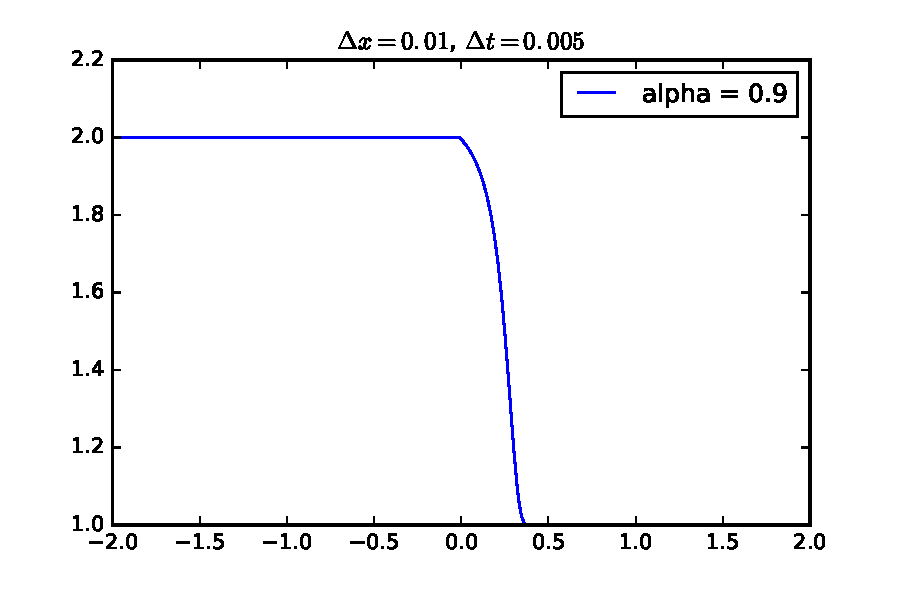
\includegraphics[width=1\textwidth]{frac_time/sta_3} \\
			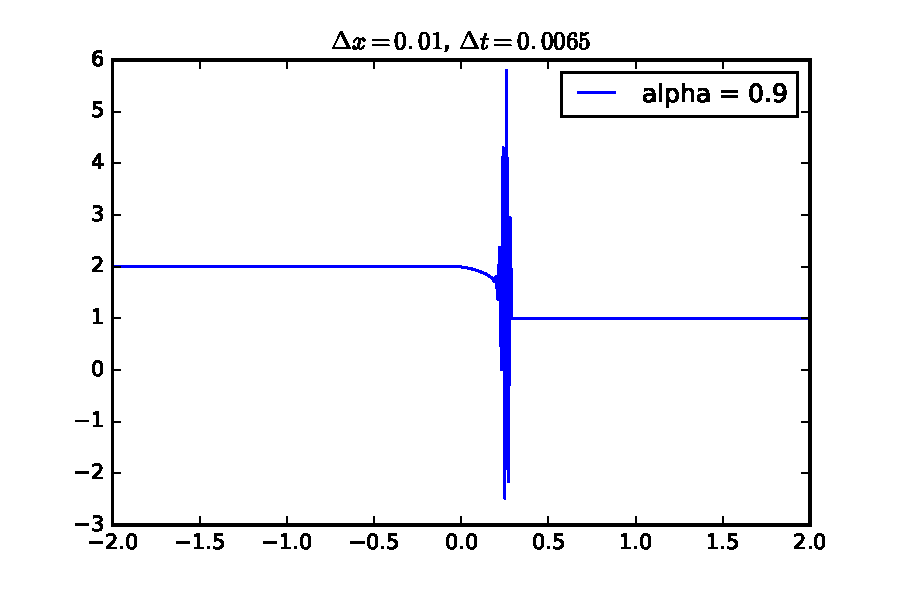
\includegraphics[width=1\textwidth]{frac_time/usta_3}
		\end{minipage}
	}
	\bicaption[sta_ex1]{稳定性条件的测试。(a) $\alpha = 0.7$. 上:当$\Delta t = 0.0008$时格式收敛。 下: 当$\Delta t = 0.00135$时格式发散。(b) $\alpha = 0.8$。上:当$\Delta t = 0.002$时格式收敛。下:当$\Delta t = 0.0035$时格式发散。(c) $\alpha = 0.9$。上:当$\Delta t = 0.005$时格式收敛。下:当$\Delta t = 0.0065$时格式发散。}{稳定性条件的测试。(a) $\alpha = 0.7$. 上:当$\Delta t = 0.0008$时格式收敛。 下: 当$\Delta t = 0.00135$时格式发散。(b) $\alpha = 0.8$。上:当$\Delta t = 0.002$时格式收敛。下:当$\Delta t = 0.0035$时格式发散。(c) $\alpha = 0.9$。上:当$\Delta t = 0.005$时格式收敛。下:当$\Delta t = 0.0065$时格式发散。}{Fig}{The stability condition test. (a) $\alpha = 0.7$. Up: scheme converges when $\Delta t = 0.0008$. Below: scheme diverges when $\Delta t = 0.00135$. (b) $\alpha = 0.8$. Up: scheme converges when $\Delta t = 0.002$. Below: scheme diverges when $\Delta t = 0.0035$. (c) $\alpha = 0.9$. Up: scheme converges when $\Delta t = 0.005$. Below: scheme diverges when $\Delta t = 0.0065$. 
	%\zz{don't use subcaption and caption at this same time... just use caption.}
	}
	% \label{sta_ex1}
\end{figure}


\subsubsection{二阶格式的收敛性和稳定性测试}	
%\zz{make the two changes as in the first order test. CFL $\Delta t$ and the caption.}
% In this part we basically repeat the numerical tests we did in the first order case. For the convergence test, we still fix $\Delta t = 0.0001$ and compute the solution at time $T = 0.2$. Due to the use of the limiters, the accuracy of MUSCL schemes may degrade to first order locally. For simplicity, we choose to use a continuous initial condition for the accuracy test,
在这一部分我们基本上重复了我们在一阶格式中进行的数值测试。对于收敛测试,我们仍然固定$ \Delta t = 0.0001 $,并在时间$ T = 0.2 $计算解。 由于限制器的使用,MUSCL方案的准确性可能会降到局部一阶。 为了简单起见,我们选择使用连续的初始条件进行精度测试,
\begin{equation}
u(x, 0) = e^{-10 x^2} + 1
\end{equation}
\begin{figure}[htbp]
	\centering
	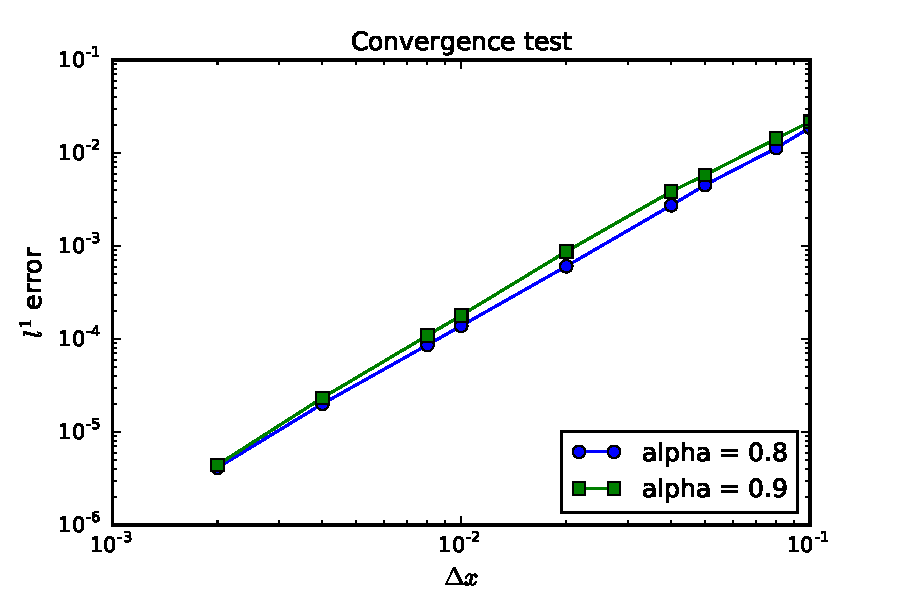
\includegraphics[width=0.8\textwidth]{frac_time/2conv_ex}
	\bicaption[fig_conv_ex2]{收敛性测试表明为$\Delta x$的二阶收敛。}{收敛性测试表明为$\Delta x$的二阶收敛。}{Fig}{Convergence test shows it is a second order scheme in $\Delta x$.}
	%\label{fig_conv_ex1}
\end{figure}
从log-log图\ref{fig_conv_ex2}中可以看出这是一个二阶格式。

稳定性测试如同前一节一样,结果显示在图\ref{sta_ex2}中。
\begin{figure}
	\centering
	\subfigure{
		\begin{minipage}[b]{0.305\textwidth}
			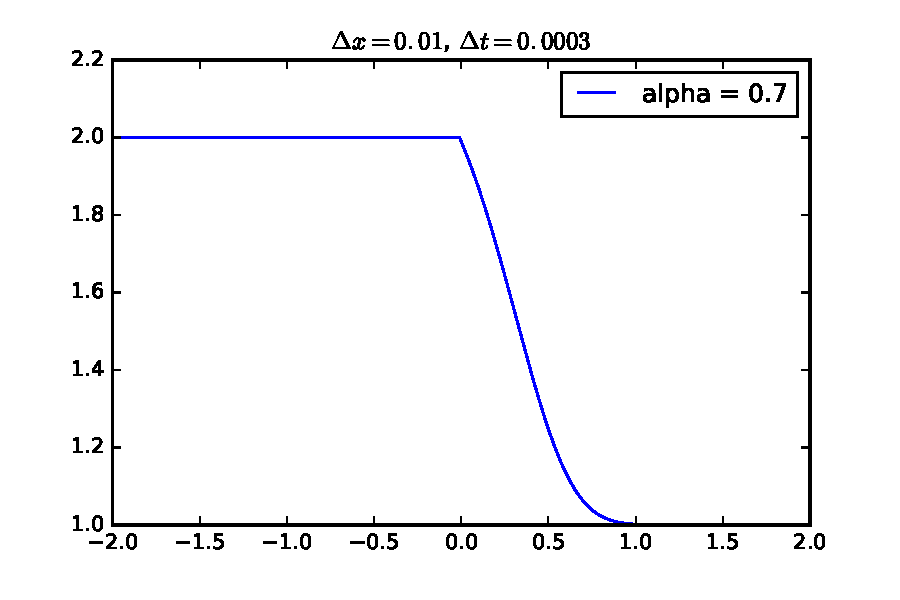
\includegraphics[width=1\textwidth]{frac_time/2sta_1} \\
			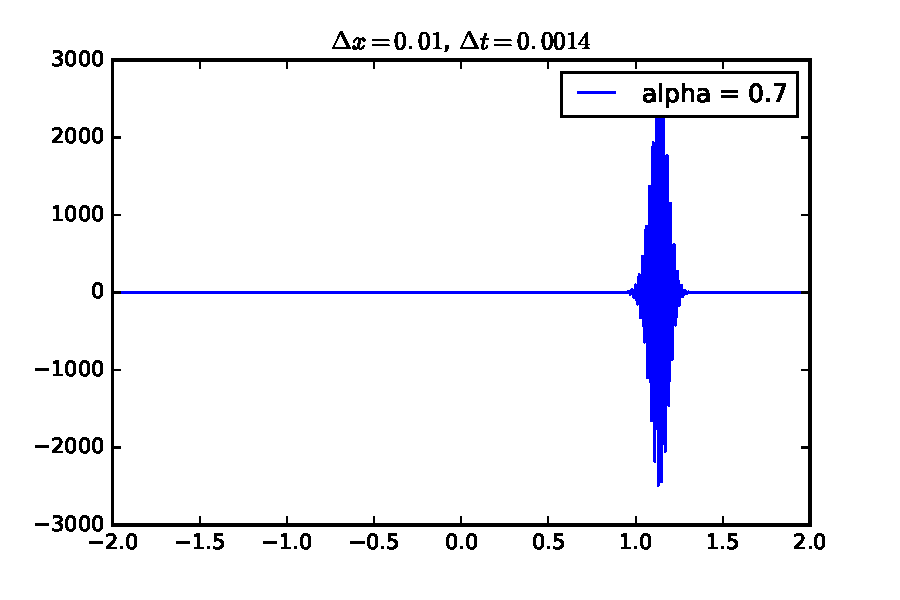
\includegraphics[width=1\textwidth]{frac_time/2usta_1}
		\end{minipage}
	}
	\subfigure{
		\begin{minipage}[b]{0.305\textwidth}
			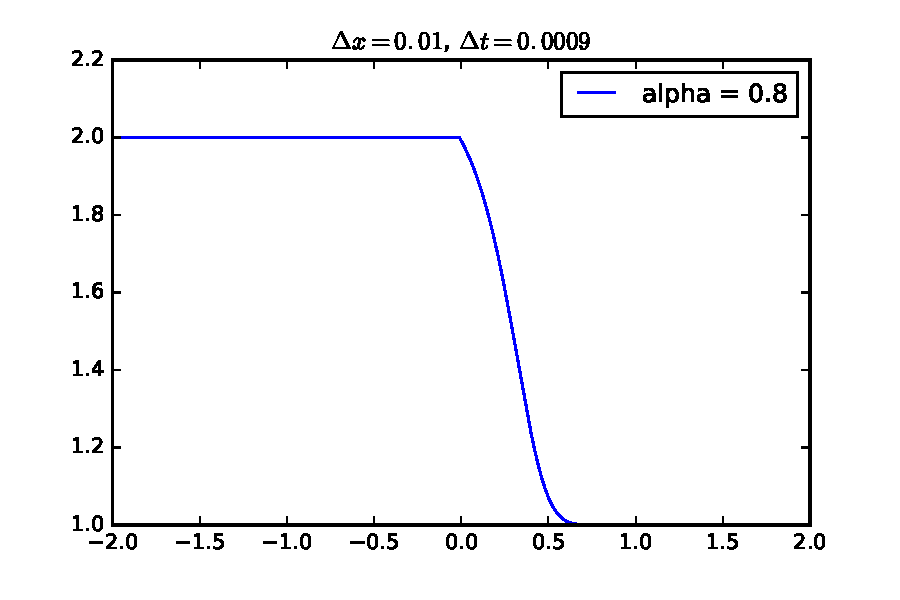
\includegraphics[width=1\textwidth]{frac_time/2sta_2} \\
			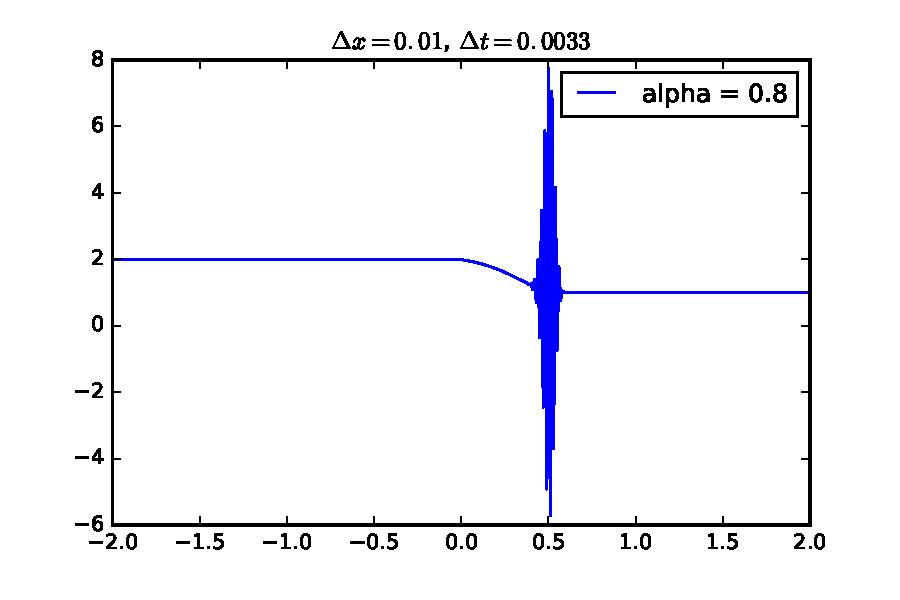
\includegraphics[width=1\textwidth]{frac_time/2usta_2}
		\end{minipage}
	}
	\subfigure{
		\begin{minipage}[b]{0.305\textwidth}
			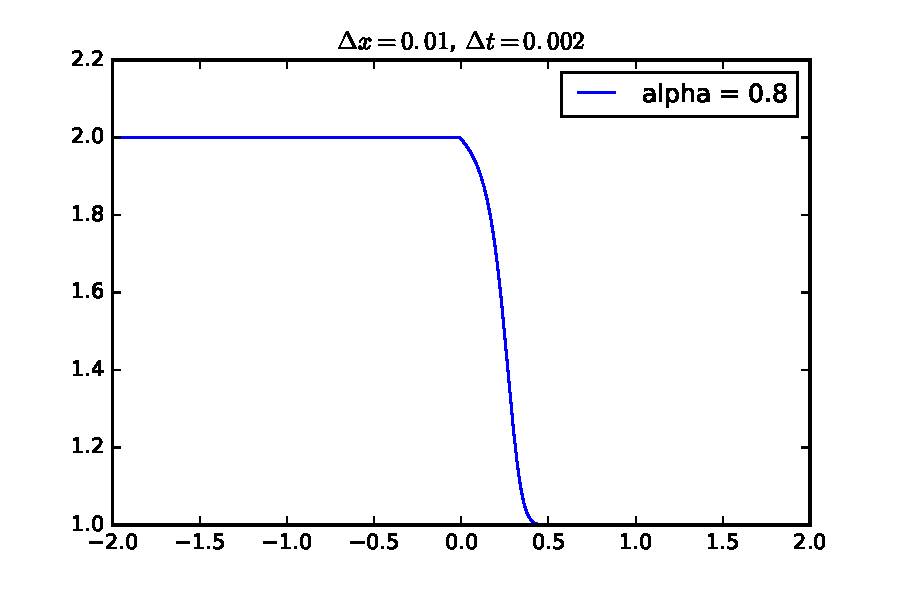
\includegraphics[width=1\textwidth]{frac_time/2sta_3} \\
			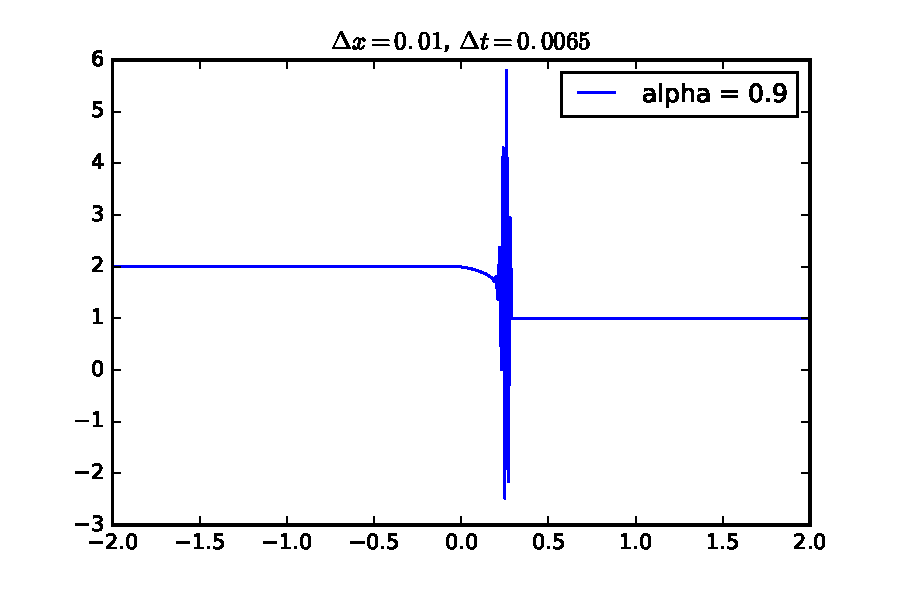
\includegraphics[width=1\textwidth]{frac_time/2usta_3}
		\end{minipage}
	}
	\bicaption[sta_ex2]{稳定性条件的测试。(a) $\alpha = 0.7$. 上:当$\Delta t = 0.0003$时格式收敛。 下: 当$\Delta t = 0.0014$时格式发散。(b) $\alpha = 0.8$。上:当$\Delta t = 0.0009$时格式收敛。下:当$\Delta t = 0.0033$时格式发散。(c) $\alpha = 0.9$。上:当$\Delta t = 0.002$时格式收敛。下:当$\Delta t = 0.0065$时格式发散。}{稳定性条件的测试。(a) $\alpha = 0.7$. 上:当$\Delta t = 0.0003$时格式收敛。 下: 当$\Delta t = 0.0014$时格式发散。(b) $\alpha = 0.8$。上:当$\Delta t = 0.0009$时格式收敛。下:当$\Delta t = 0.0033$时格式发散。(c) $\alpha = 0.9$。上:当$\Delta t = 0.002$时格式收敛。下:当$\Delta t = 0.0065$时格式发散。}{Fig}{The stability condition test. (a) $\alpha = 0.7$. Up: scheme converges when $\Delta t = 0.0003$. Below: scheme diverges when $\Delta t = 0.0014$. (b) $\alpha = 0.8$. Up: scheme converges when $\Delta t = 0.0009$. Below: scheme diverges when $\Delta t = 0.0033$. (c) $\alpha = 0.9$. Up: scheme converges when $\Delta t = 0.002$. Below: scheme diverges when $\Delta t = 0.0065$.}
	% \label{sta_ex2}
\end{figure}
同样的可以看到对$\Delta t$的强约束是的计算非常低效。

% To conclude this section, we remark that, we have carried out the same tests for the Burgers' equation, and similar results have been obtained, which we would skip in this paper.
总结本节,我们指出,我们对Burgers'方程进行了相同的测试,并得到了类似的结果,将在本章中略去。
%\subsubsection{The showcase of the solution}
%After the convergence test, we will give some plot of the solution to give some intuitions of this equation.
%
%Figure \ref{ex_1} shows the solution with two different types of initial condition. The equation has some damping effects that make the solution more smoother as time evolves.
%\begin{figure}[htbp]
%	\includegraphics[width=0.5\textwidth]{fig/1}
%	\includegraphics[width=0.5\textwidth]{fig/2}
%	\caption{Solution at $T=0.2$ with $\alpha = 0.8$, $a = 1$, $\Delta x = 0.01$ and $\Delta t = 10^{-4}$. Left: initial data $u_0(x) = 0.5\sin(1.5\pi x) + 1.5$; Right: initial data $u_0(x) = 2$ when $x < 0$ and $u_0(x) = 1$ when $x > 0$.}
%	\label{ex_1}
%\end{figure}
%
%Next we will give an example of burgers' equation:
%\begin{equation}
%\partial^\alpha_t u + \frac{1}{2}\partial_x (u^2) = 0, 
%\end{equation}
%using our first order explicit upwind scheme. The result is shown in Figure \ref{ex_bur}, also with a smooth initial condition and discontinuous initial condition.
%\begin{figure}[htbp]
%	\includegraphics[width=0.5\textwidth]{fig/7}
%	\includegraphics[width=0.5\textwidth]{fig/8}
%	\caption{Solution at $T=0.2$ with $\alpha = 0.8$, $\Delta x = 0.01$ and $\Delta t = 10^{-4}$. Left: initial data $u_0(x) = 0.5\sin(1.5\pi x) + 1.5$; Right: initial data $u_0(x) = 2$ when $x < 0$ and $u_0(x) = 1$ when $x > 0$.}
%	\label{ex_bur}
%\end{figure}
%We will provide more examples of burgers' equation in next section.

\subsection{隐式格式的例子}
% In the previous section, we show that it is nearly infeasible to use an explicit scheme for small $\alpha$. Due to the restricted CFL conditions, an explicit scheme is extremely inefficient especially when $\alpha \rightarrow 0$. which motivates us to use an implicit scheme instead. By using an implicit scheme, we can conduct more numerical tests to explore more about the conservation law with the Caputo derivative.
在上一节中,我们说明了对于小的$ \alpha $使用显式方案几乎是不可行的。 由于CFL条件的限制,一个显式格式是非常低效的,特别是当$ \alpha \rightarrow 0 $。 这促使我们改用隐式格式。 通过使用隐式格式,我们可以进行更多的数值测试,以对Caputo导数的守恒律作更多地了解。

\subsubsection{隐式格式的收敛性}
%\zz{this section is still very immature... need explanations and rework. For the stability test, you need to fix sufficiently small $\Delta x$ and increase $\Delta t$. And details of the numerical tests need to be added.}

% In this subsection, we will test the convergence of implicit upwind scheme. All the configurations for scalar convection equation are the same as previous section. We still fix $\Delta x=0.01$ and since we expect this scheme to be unconditionally stable, we also choose $\alpha=0.2$ which is the case we cannot afford in the explicit case. For the stability test, we choose $\Delta t=0.01, 0.02, 0.04, 0.06, 0.08$ which is $O(\Delta x)$ as shown in Figure \ref{sta_conv_im} left. For the convergence test, we can now fix $\Delta t=0.01$, thanks to the unconditionally stable feature and a first order convergence in space is observed (see Figure \ref{sta_conv_im} right).  %\zz{provide $\Delta x$ information.}
在本小节中,我们将测试隐性迎风格式的收敛性。标量对流方程的所有参数与上一节相同。 我们仍然固定$ \Delta x = 0.01 $,由于我们预计这个格式是无条件稳定的,所以我们选择$ \alpha = 0.2 $,这是我们在显式的情况下做不到的。 对于稳定性测试,我们选择$ \Delta t = 0.01,0.02,0.04,0.06,0.08 $,这是$ O(\Delta x)$,如图\ref {sta_conv_im}所示。 对于收敛测试,我们现在可以固定$ \Delta t = 0.01 $,这得益于无条件稳定的特征,并且观察到空间中的一阶收敛(见图\ref{sta_conv_im} 右)。

\begin{figure}[htbp]
	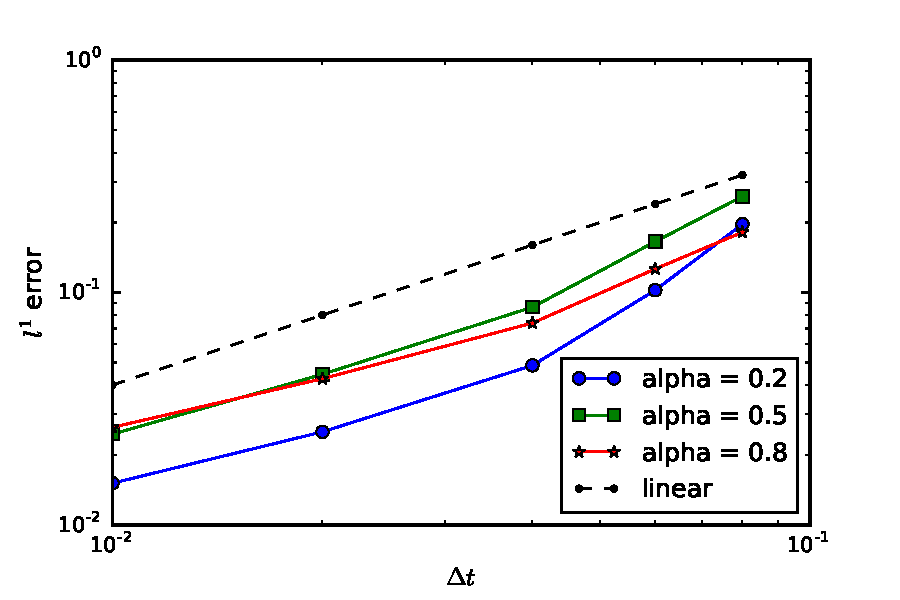
\includegraphics[width=0.5\textwidth]{frac_time/sta_im_rev}
	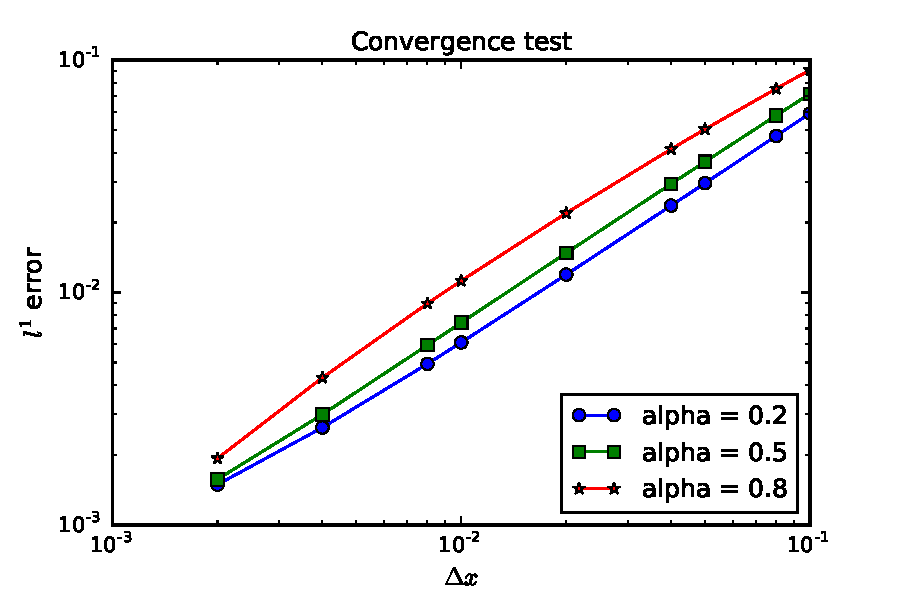
\includegraphics[width=0.5\textwidth]{frac_time/conv_im}
	\bicaption[sta_conv_im]{对于不同的$\alpha$的线性对流方程的隐式迎风格式。左:稳定性测试;右:关于$\Delta x$的收敛性测试。}{对于不同的$\alpha$的线性对流方程的隐式迎风格式。左:稳定性测试;右:关于$\Delta x$的收敛性测试。}{Fig}{Implicit upwind scheme for the linear advection equation with different $\alpha$. Left: stability test. Right: convergence test in $\Delta x$.}
	% \label{sta_conv_im}
\end{figure}

% This constraint-free stability feature also allows us to run a test of solving nonlinear fractional equations. Here we test a Burgers' equation with the Caputo derivative:
无条件稳定的特性也使我们解非线性的守恒律方程,这里我们测试带Caputo导数的Burges'方程:
\begin{equation}\label{eq_burgers}
\begin{cases}
\partial^\alpha_t u + u\partial_x u = 0, \\
u(x, 0) = -\sin(\pi x).
\end{cases}
\end{equation}
% with fixed $\alpha = 0.2, 0.5, 0.8$. Same as above, for the stability test we fix $\Delta x=0.01$ and increase $\Delta t$; for the convergence test we fix $\Delta t=0.01$ and increase $\Delta x$. The results are shown in Figure \ref{sta_conv_bur}. We remark that, in the stability test, the numerical error decreases in proportion to $\Delta t$ until the spatial error becomes dominant, which explains the flat error curve for small $\Delta t$. 
对于固定的$\alpha = 0.2, 0.5, 0.8$。和前面一样,稳定性测试我们固定$\Delta x=0.01$,让$\Delta t$增加;收敛性测试我们固定$\Delta t=0.01$,让$\Delta x$增加。结果显示在图\ref{sta_conv_bur}。在稳定性测试中,数值误差正比于$\Delta t$的减少知道空间误差占主要地位,这解释了对于小的$\Delta t$较平的误差曲线。
 
\begin{figure}[htbp]
	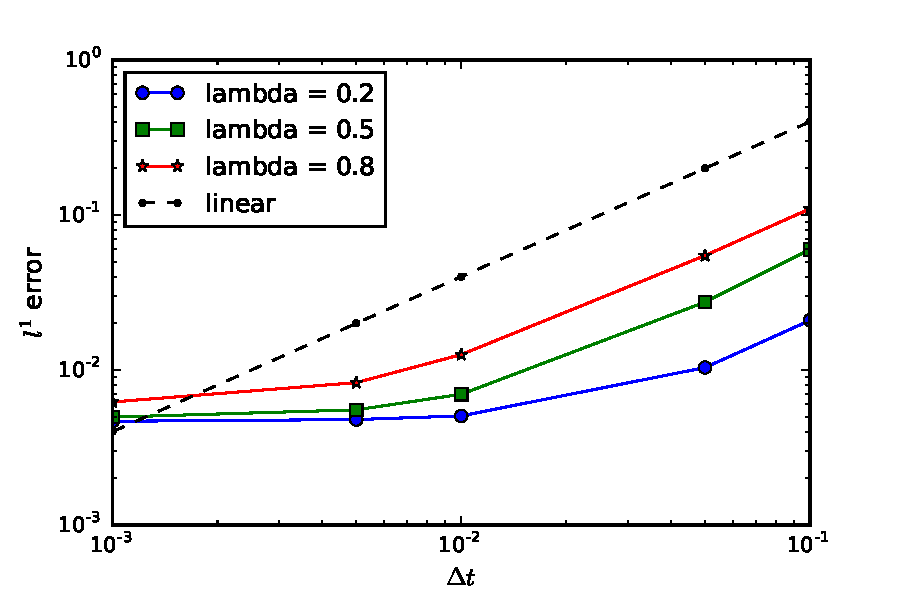
\includegraphics[width=0.5\textwidth]{frac_time/sta_im_bur_0}
	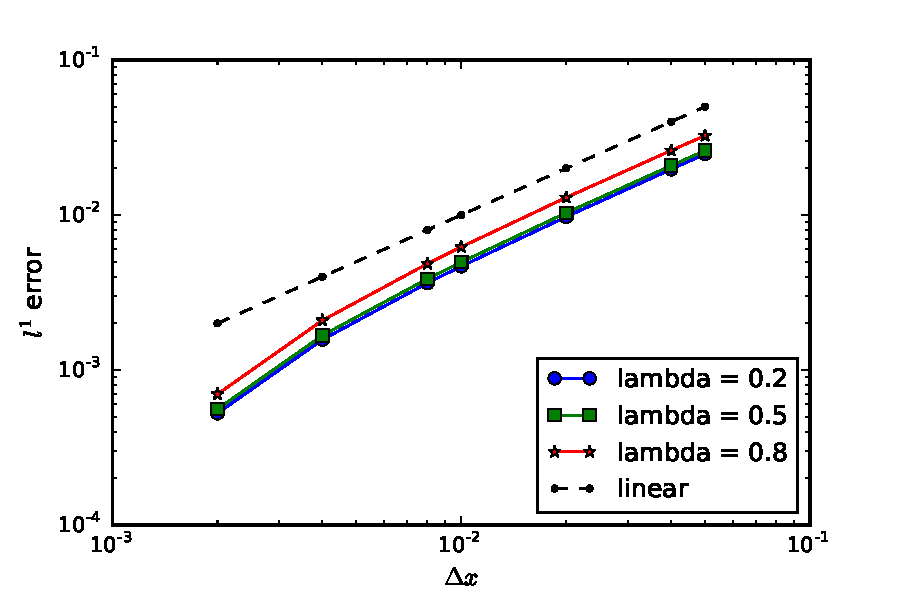
\includegraphics[width=0.5\textwidth]{frac_time/conv_im_bur_0}
	\bicaption[sta_conv_bur]{Burgers'方程的隐式迎风格式。左:稳定性测试;右:关于$\Delta x$的收敛性测试。}{Burgers'方程的隐式迎风格式。左:稳定性测试;右:关于$\Delta x$的收敛性测试。}{Fig}{Implicit upwind scheme for the Burgers' equation. Left: stability test. Right: convergence test in $\Delta x$.}
	% \label{sta_conv_bur}
\end{figure}

\subsubsection{数值实验:理解记忆效应}
% As we can see, since the implicit scheme is efficient and stable for conservation laws with the Caputo derivative, we will use this scheme to investigate these equations. We will give several tests in this section. 
我们可以看出,由于隐式格式对于使用Caputo导数的守恒定律是有效和稳定的,我们将使用该格式来研究这些方程。将在本节中给出几个测试。

% First we show the solutions with different $\alpha$'s for the advection equation and the Burgers' equation respectively. In Figure \ref{as} left, we observe that the solutions at discontinuous point exhibit convergent behavior as $\alpha \rightarrow 1$, finally converges to the solution when $\alpha = 1$ which is the standard convection equation.
% For the Burgers' equation, the same behavior is shown as in Figure \ref{as} right.
首先,我们分别用对流方程和Burgers'方程显示在不同的$\alpha $下的解。 在图\ref{as}(左)中,我们观察到间断的解表现的收敛行为,当$\alpha \rightarrow 1 $时,最终收敛于当$ \alpha = 1 $时标准对流方程的解,
对于Burgers'方程,同样的行为如图\ref{as}(右)所示。
\begin{figure}[htbp]
	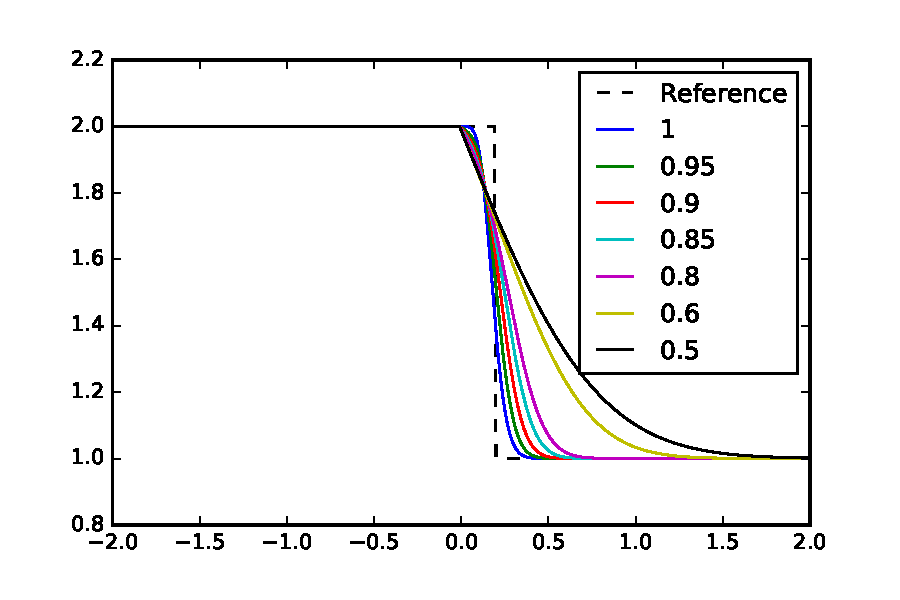
\includegraphics[width=0.5\textwidth]{frac_time/alpha}
	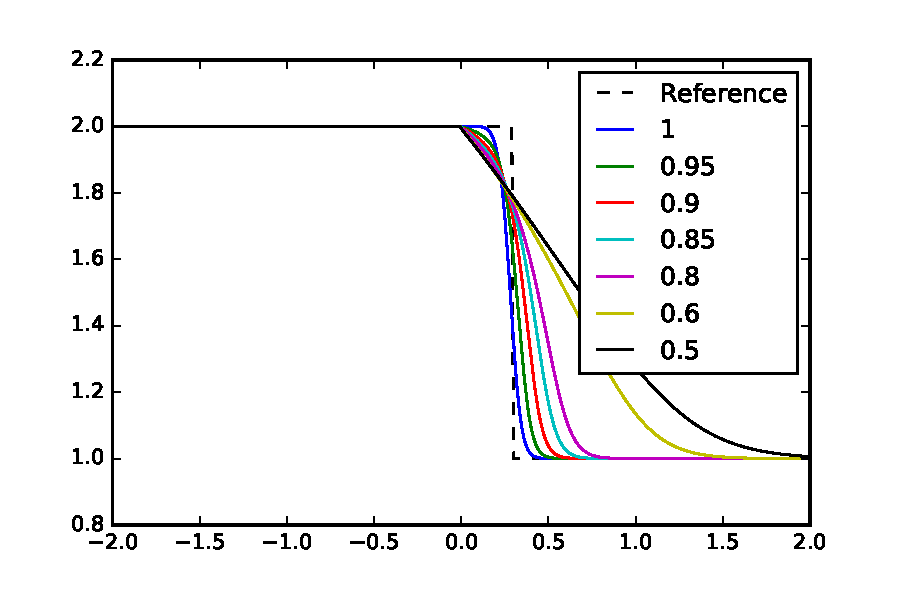
\includegraphics[width=0.5\textwidth]{frac_time/alpha2}
	\bicaption[as]{由隐式迎风格式计算的不同的$\alpha$的解,$T=0.2$,$a = 1$,$\Delta t = \Delta x = 0.01$。左:线性对流方程;右:Burgers方程。}{由隐式迎风格式计算的不同的$\alpha$的解,$T=0.2$,$a = 1$,$\Delta t = \Delta x = 0.01$。左:线性对流方程;右:Burgers方程。}{Fig}{Solutions at $T=0.2$ with different $\alpha$, $a = 1$, $\Delta t = \Delta x = 0.01$, by the implicit upwind method. Left: linear advection equation. Right: Burgers' equation}
	% \label{as}
\end{figure}

% Next we consider the case of inhomogeneous memory effect, i.e., when $\alpha$ depends on $x$ and $t$. In the linear convection case, we consider
接下来考虑不均匀的记忆效应,即$\alpha$依赖于$x$和$t$。在线性对流的情况,考虑
\begin{equation}
\alpha(x, \lambda) = 1 - \lambda\exp(-30 x^2 - 7000\times (0.5)^{12}),
\end{equation}
初值为
\begin{equation}
u(x, 0) = 
\begin{cases}
0.5\cos(\pi(2x + 4)) + 0.5,  &\quad x\in[-1.5, -0.5] \\
0, &\quad \mbox{其他}
\end{cases}
\end{equation}
在图\ref{1},图\ref{2},图\ref{3}中,展示了不同$\alpha(x, t)$下的解。观察到由记忆效应导致的垂直方向的压缩和水平方向的扩展。
\begin{figure}[H]
	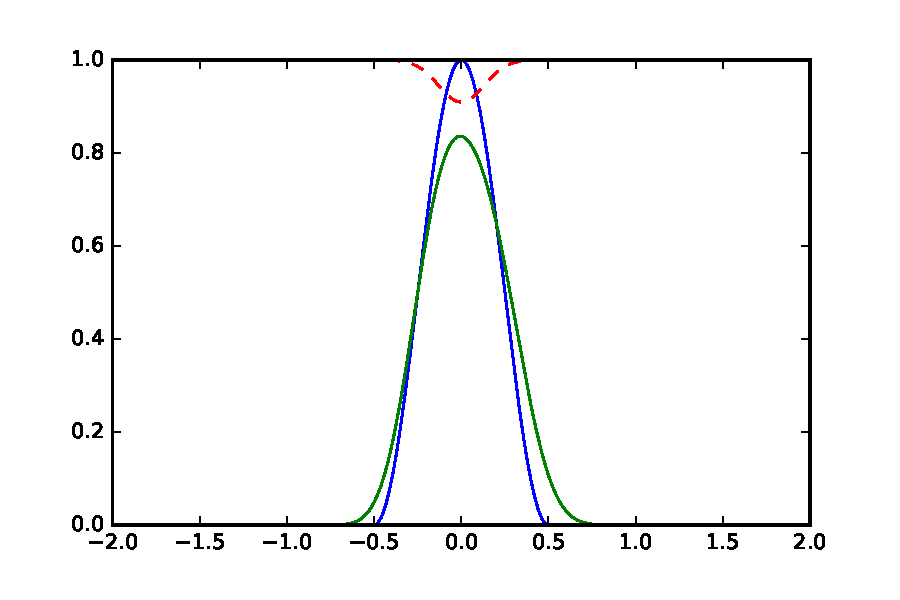
\includegraphics[width=0.5\textwidth]{frac_time/conv_1}
	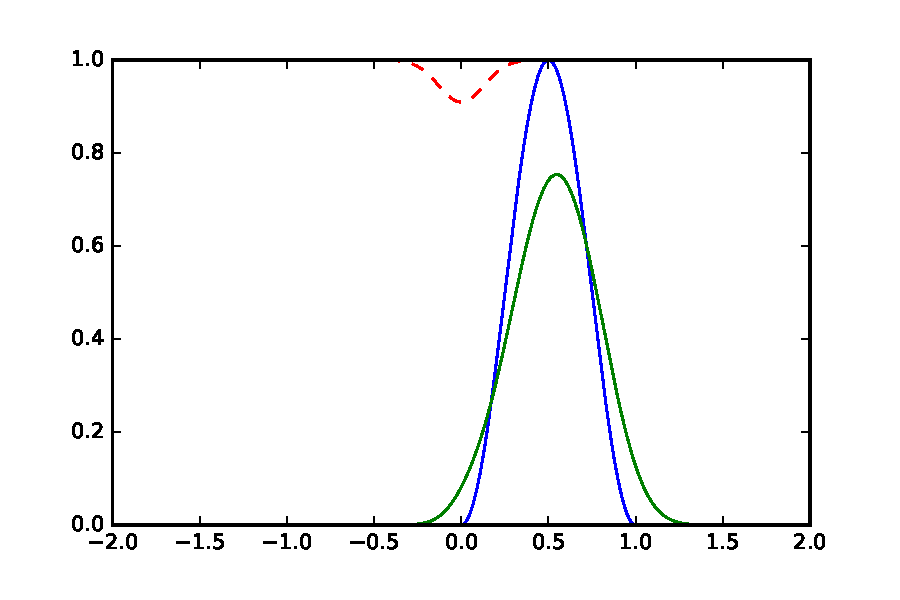
\includegraphics[width=0.5\textwidth]{frac_time/conv_2}
	\bicaption[1]{左:数值解(绿线)在$T = 1$及$\lambda = 0.5$(虚线)和精确解在$T = 1$,$\alpha = 1$(蓝线)。右:数值解(绿线)在$T = 1.5$及$\lambda = 0.5$(虚线)和精确解在$T = 1.5$,$\alpha = 1$(蓝线)。虚线为对于相应的$\lambda$下的$\alpha(x,\lambda)$。}{左:数值解(绿线)在$T = 1$及$\lambda = 0.5$(虚线)和精确解在$T = 1$,$\alpha = 1$(蓝线)。右:数值解(绿线)在$T = 1.5$及$\lambda = 0.5$(虚线)和精确解在$T = 1.5$,$\alpha = 1$(蓝线)。虚线为对于相应的$\lambda$下的$\alpha(x,\lambda)$。}{Fig}{Left: solution (green line) at $T = 1$ with $\lambda = 0.5$ (dash line) and exact solution with $T = 1$, $\alpha = 1$ (blue line). Right: solution (green line) at $T = 1.5$ with $\lambda = 0.5$ (dash line) and exact solution with $T = 1.5$, $\alpha = 1$ (blue line). Dash line is $\alpha(x, \lambda)$ with corresponding $\lambda$s.}
	% \label{1}
\end{figure}
\begin{figure}[H]
	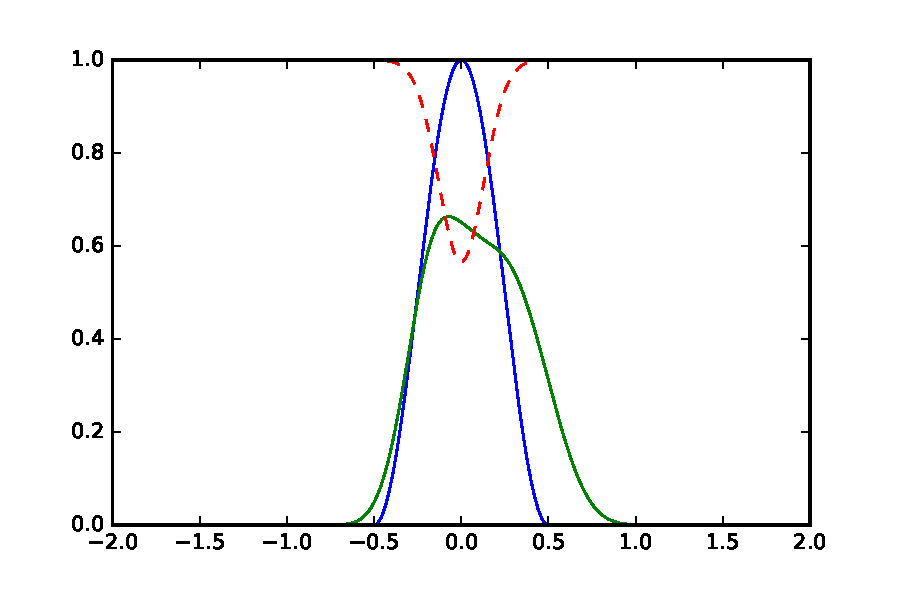
\includegraphics[width=0.5\textwidth]{frac_time/conv_3}
	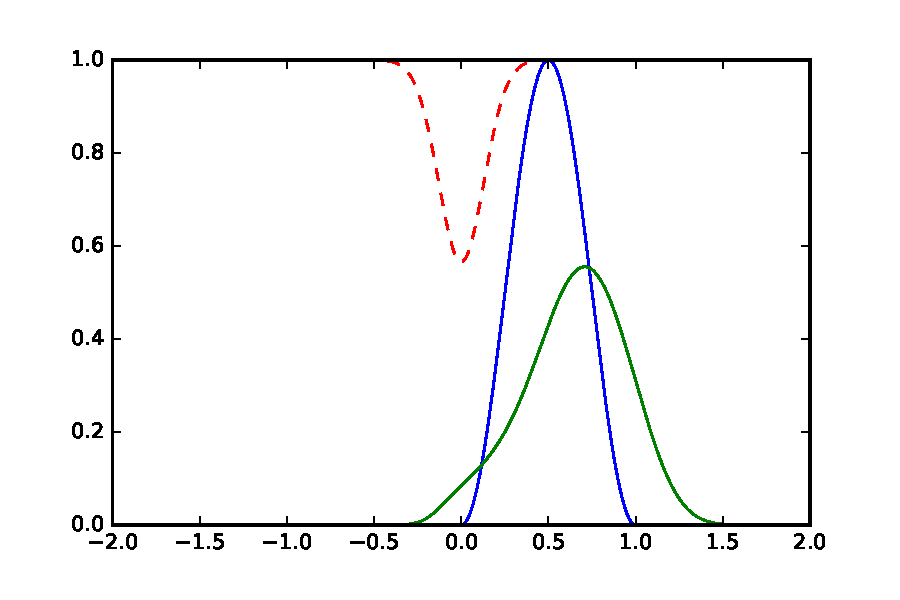
\includegraphics[width=0.5\textwidth]{frac_time/conv_4}
	\bicaption[2]{左:数值解(绿线)在$T = 1$及$\lambda = 2.4$(虚线)和精确解在$T = 1$,$\alpha = 1$(蓝线)。右:数值解(绿线)在$T = 1.5$及$\lambda = 2.4$(虚线)和精确解在$T = 1.5$,$\alpha = 1$(蓝线)。虚线为对于相应的$\lambda$下的$\alpha(x,\lambda)$。}{左:数值解(绿线)在$T = 1$及$\lambda = 2.4$(虚线)和精确解在$T = 1$,$\alpha = 1$(蓝线)。右:数值解(绿线)在$T = 1.5$及$\lambda = 2.4$(虚线)和精确解在$T = 1.5$,$\alpha = 1$(蓝线)。虚线为对于相应的$\lambda$下的$\alpha(x,\lambda)$。}{Fig}{Left: solution (green line) at $T = 1$ with $\lambda = 2.4$ (dash line) and exact solution with $T = 1$, $\alpha = 1$ (blue line). Right: solution (green line) at $T = 1.5$ with $\lambda = 2.4$ (dash line) and exact solution with $T = 1.5$, $\alpha = 1$ (blue line). Dash line is $\alpha(x, \lambda)$ with corresponding $\lambda$s.}
	% \label{2}
\end{figure}
\begin{figure}[H]
	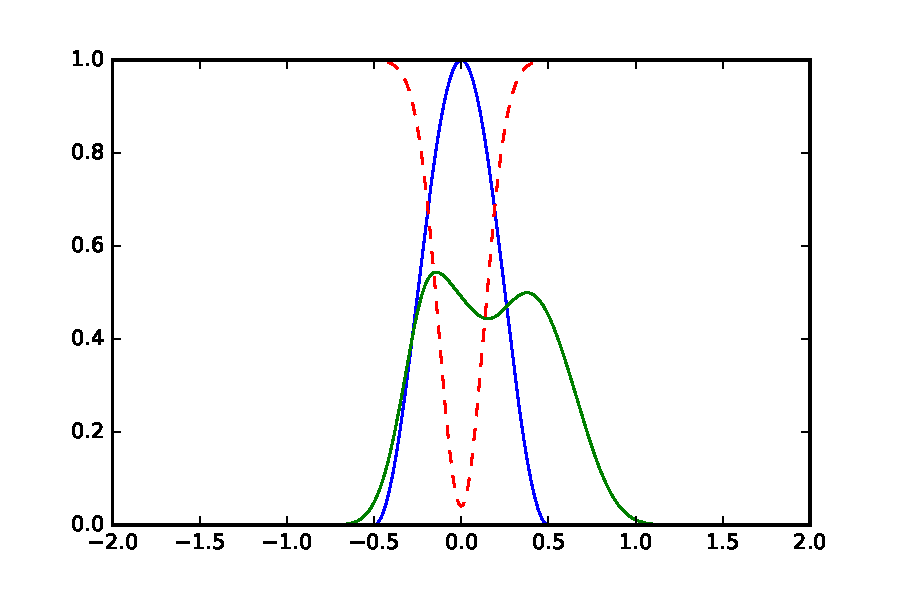
\includegraphics[width=0.5\textwidth]{frac_time/conv_5}
	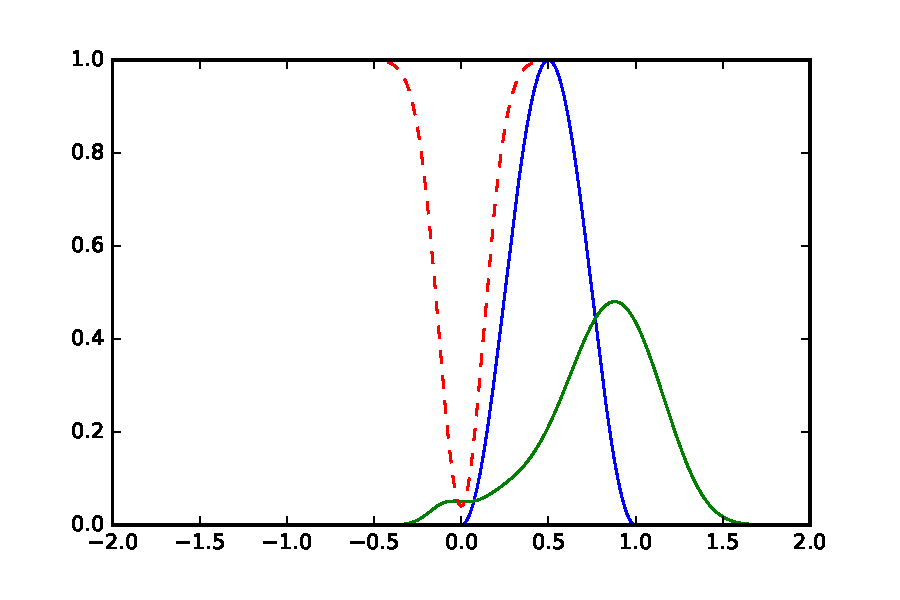
\includegraphics[width=0.5\textwidth]{frac_time/conv_6}
	\bicaption[3]{左:数值解(绿线)在$T = 1$及$\lambda = 5.3$(虚线)和精确解在$T = 1$,$\alpha = 1$(蓝线)。右:数值解(绿线)在$T = 1.5$及$\lambda = 5.3$(虚线)和精确解在$T = 1.5$,$\alpha = 1$(蓝线)。虚线为对于相应的$\lambda$下的$\alpha(x,\lambda)$。}{左:数值解(绿线)在$T = 1$及$\lambda = 5.3$(虚线)和精确解在$T = 1$,$\alpha = 1$(蓝线)。右:数值解(绿线)在$T = 1.5$及$\lambda = 5.3$(虚线)和精确解在$T = 1.5$,$\alpha = 1$(蓝线)。虚线为对于相应的$\lambda$下的$\alpha(x,\lambda)$。}{Fig}{Left: solution (green line) at $T = 1$ with $\lambda = 5.3$ (dash line) and exact solution with $T = 1$, $\alpha = 1$ (blue line). Right: solution (green line) at $T = 1.5$ with $\lambda = 5.3$ (dash line) and exact solution with $T = 1.5$, $\alpha = 1$ (blue line). Dash line is $\alpha(x, \lambda)$ with corresponding $\lambda$s.}
	% \label{3}
\end{figure}

最后我们考虑Burgers'方程(\ref{eq_burgers}),
% \begin{equation}
% \begin{cases}
% \partial^\alpha_t u + u\partial_x u = 0, \\
% u(x, 0) = -\sin(\pi x).
% \end{cases}
% \end{equation}
其中$\alpha_1(x, t) = 1 - 0.9\exp(-8|x| - 7000(t - 0.8)^{12})$及$\alpha_2(x, t) = 1$,这个例子和Karniadakis的文章\citen{Karniadakis:2013coba}中的一样。然而,它们文章中得到的解受到Gibbs现象的破坏,这是由于它们在间断处使用了伪谱方法。这里,我们的结果是没有数值振荡的,同时也观察到了压缩效应,见图\ref{bur_1}和图\ref{bur_2}。
\begin{figure}[H]
	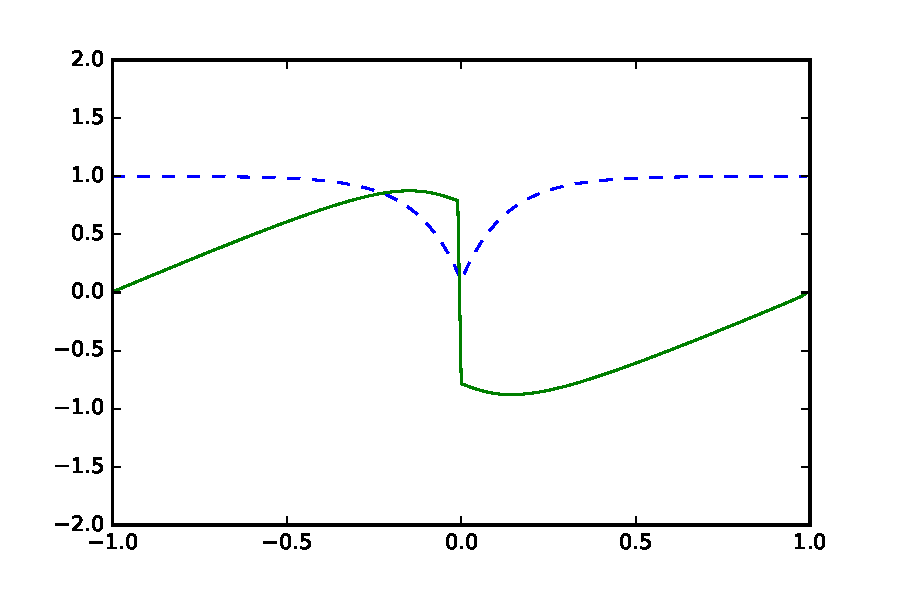
\includegraphics[width=0.5\textwidth]{frac_time/burgers_1}
	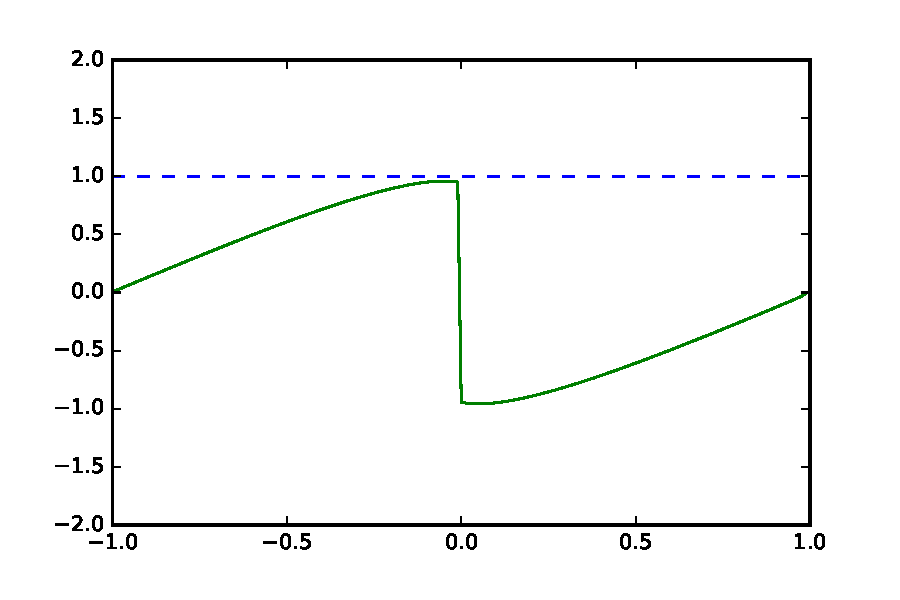
\includegraphics[width=0.5\textwidth]{frac_time/burgers_2}
	\bicaption[bur_1]{左:数值解(实线)在$T=0.5$及$\alpha = \alpha_1(x,t)$ (虚线),$\Delta t = \Delta x = 0.01$。右:数值解(实线)在$T=0.5$及$\alpha = 1$,$\Delta t = \Delta x = 0.01$。由隐式迎风格式得到。}{左:数值解(实线)在$T=0.5$及$\alpha = \alpha_1(x,t)$ (虚线),$\Delta t = \Delta x = 0.01$。右:数值解(实线)在$T=0.5$及$\alpha = 1$,$\Delta t = \Delta x = 0.01$。由隐式迎风格式得到。}{Fig}{Left: solution (solid line) at $T=0.5$ with $\alpha = \alpha_1(x,t)$ (dash line), $\Delta t = \Delta x = 0.01$. Right: solution (solid line) at $T=0.5$ with $\alpha = 1$, $\Delta t = \Delta x = 0.01$ by using the implicit upwind method with fast sweeping method~\citen{zhao:2003}.}
	% \label{bur_1}
\end{figure}
\begin{figure}[H]
	\centering
	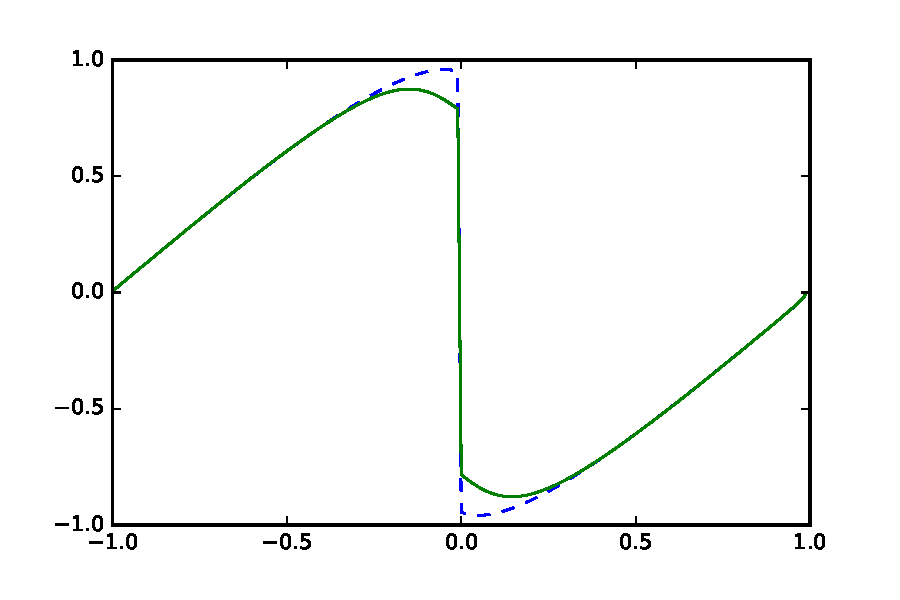
\includegraphics[width=0.8\textwidth]{frac_time/burgers_3}
	\bicaption[bur_2]{左:数值解(实线)在$T=0.5$及$\alpha = \alpha_1(x,t)$ (虚线),$\Delta t = \Delta x = 0.01$。右:数值解(实线)在$T=0.5$及$\alpha = 1$,$\Delta t = \Delta x = 0.01$。由隐式迎风格式得到。}{左:数值解(实线)在$T=0.5$及$\alpha = \alpha_1(x,t)$ (虚线),$\Delta t = \Delta x = 0.01$。右:数值解(实线)在$T=0.5$及$\alpha = 1$,$\Delta t = \Delta x = 0.01$。由隐式迎风格式得到。}{Fig}{Solution (green solid line) at $T=0.5$ with $\alpha = \alpha_1(x,t)$ and solution (blue dash line) at $T=0.5$ with $\alpha = 1$, $\Delta t = \Delta x = 0.01$ by using the implicit upwind method with fast sweeping method~\citen{zhao:2003}.}
	% \label{bur_2}
\end{figure}

\section{本章总结与展望}

本章中,我们考虑了带有Caputo(分数阶)时间导数的守恒律方程,提出了相应的一阶、二阶显式、隐式迎风格式,对于稳定性和TVD特性进行了分析。我们通过大量的数值实验,包括Burgers方程等来说明我们的格式的可行性。同时,利用构造的格式来研究分数阶导数带来的“记忆效应”的现象,加深了对这类方程的理解。

对于带有分数阶的PDE,是近年来非常热门的研究领域,无论在分析还是在计算方法的研究上,都非常有价值,尤其是在多空介质中的物理问题的记忆效应的研究中。然而,相关的数值分析与理论分析结果都非常有限,在未来将会对此继续进行深入的研究。

% \section*{Acknowledgments}
% The authors would like to thank Jianfeng Lu for helpful discussions. J. Liu is partially supported by KI-Net NSF RNMS grant No. 1107444 and NSF grant DMS 1514826. Z. Zhou is partially supported by RNMS11-07444 (KI-Net).  Z. Ma is partially supported by the NSF grant DMS--1522184, DMS--1107291: RNMS (KI-Net) and Natural Science Foundation of China grant 91330203.


%\bibliography{frac_bibtex}
%\end{document}